%Experiments

This chapter describes the experiments that were carried out to investigate the different components of one dimensional time reversal focusing at a defect location which is at an a prior unknown location. The components investigated include: i) detecting that a crack as occurred within the rod, ii) comparing theory to experiment for the interrogatory phase and for the first iteration of time reversal focusing, and iii) iterative focusing to achieve better a response at the defect until convergence is reached. All of the hardware and algorithms used are detailed. Code samples are given in the appendices.

\section{Hardware and Software}
The main access point to the system was a desktop pc which ran Windows XP and acted as the host computer. The power house of the entire system was a National Instruments 7853R FPGA card. This FPGA card was of PXI form factor and was housed in an NI proprietary PXI chassis which was linked to the PC via MXI cable (Figure \ref{fig:fpgaCard}). The PC contained a PCI-E card that allowed for the MXI connection. LabVIEW software with the extra real-time and FPGA modules was used to compile write and compile programs on the Windows PC. Once written and compiled to VHDL code the programs were then downloaded to the FPGA card over the MXI connection. The program execution is such that a host program runs on the desktop PC and communicates with the program running on the remote FPGA card. The time critical processes such as signal acquisition and playback are performed using the FPGA whereas the tasks that could take an arbitrary amount of time were executed on the desktop PC. The FPGA card does not provide a large amount of current and it was necessary to amplify the output signals using op-amp amplifier circuits which were capable of providing up to $30 VPP$ at $200 kHz$ (Figures \ref{fig:oneAmp} and \ref{fig:ampBox}). The interfacing of the data acquisition cables to the FPGA card was handled using an NI SCB-60 input/output box which provided screw terminal connections inside of a shielded box (Figure \ref{fig:ioBox}). The entire hardware hierarchy is shown in Figure \ref{fig:hardwareComm}. Finally, all of the data was imported into MATLAB.

\begin{figure}[ht!]
\centering
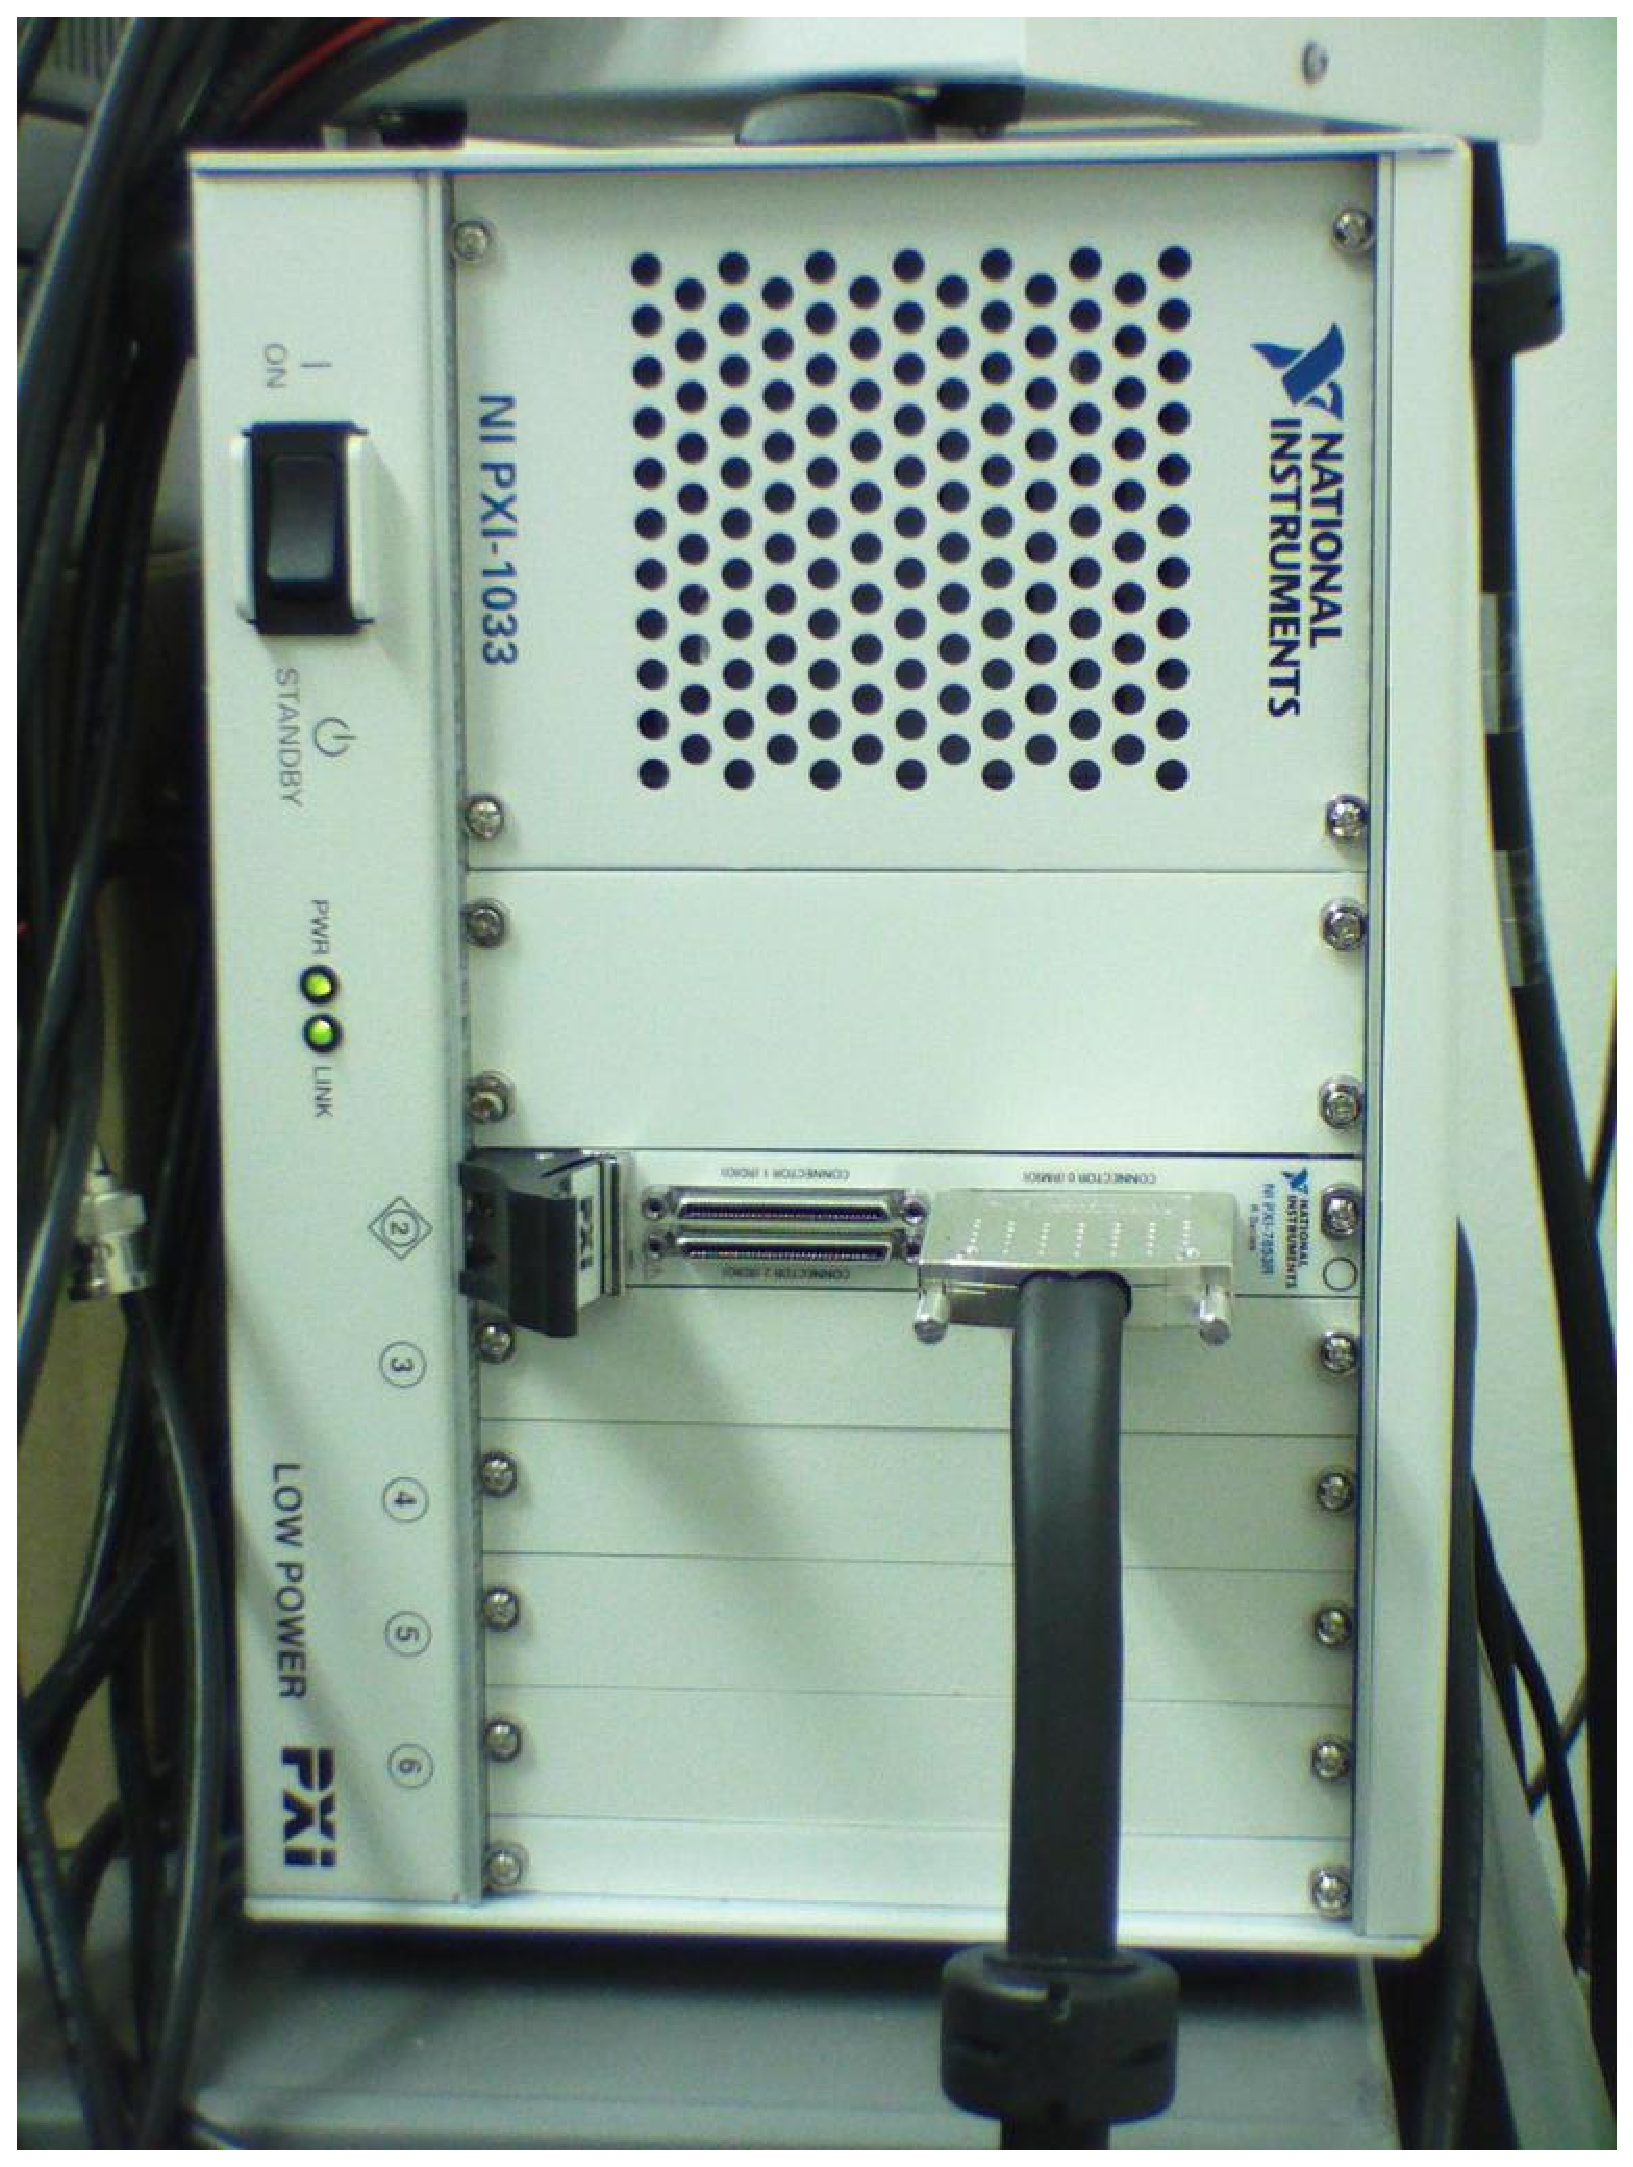
\includegraphics[width=0.6\textwidth]{eps_pics/fpgaCard}
\caption{National Instruments PXI chassis which contains the 7853R FPGA card. The 7853R is a very powerful card with a large amount of programming flexibility due to the fact that it can be programmed using a graphical language (LabVIEW) instead of needing to code directly in VHDL which can be cumbersome.
	 \label{fig:fpgaCard}} 
\end{figure}

\begin{figure}[ht!]
\centering
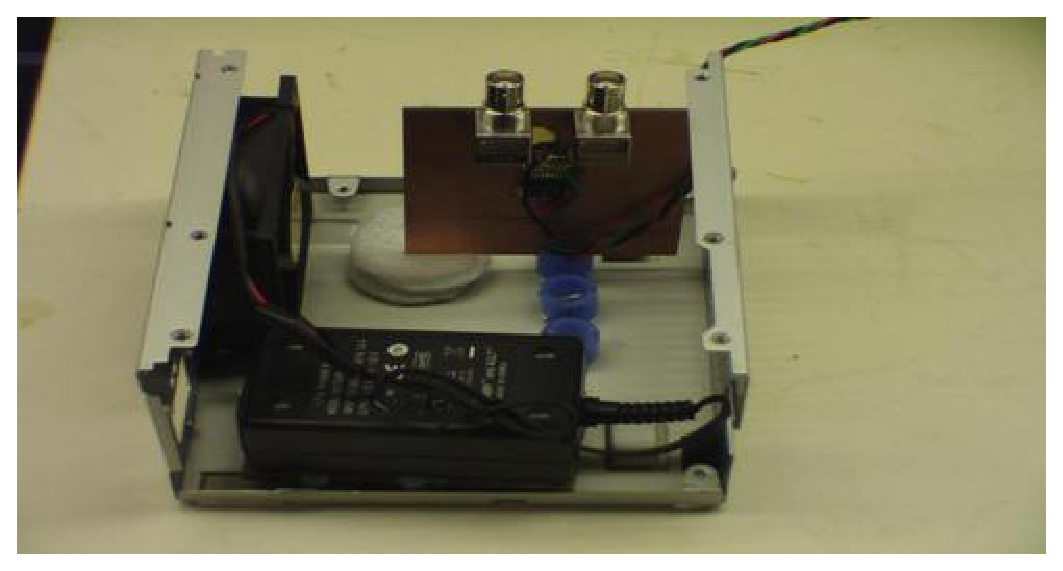
\includegraphics[width=0.7\textwidth]{eps_pics/oneAmp}
\caption{Single amplifier circuit being placed into the custom enclosure that was built from a PC power supply casing. Many thanks go to Miles Wickersham and Andy Downs for their help with designing the circuits.
	 \label{fig:oneAmp}} 
\end{figure}

\begin{figure}[ht!]
\centering
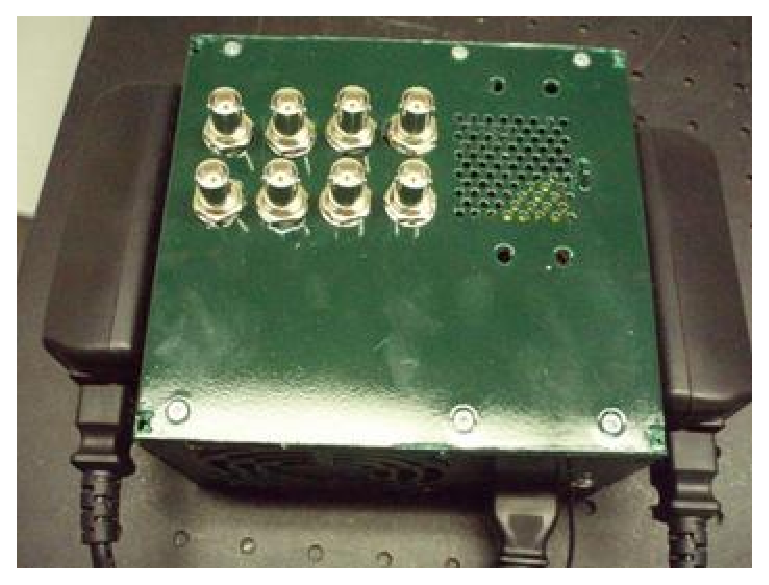
\includegraphics[width=0.7\textwidth]{eps_pics/ampBox}
\caption{Completed amplifier box containing four op-amp amplifier circuits with BNC input and output
	 \label{fig:ampBox}} 
\end{figure}

\begin{figure}[ht!]
\centering
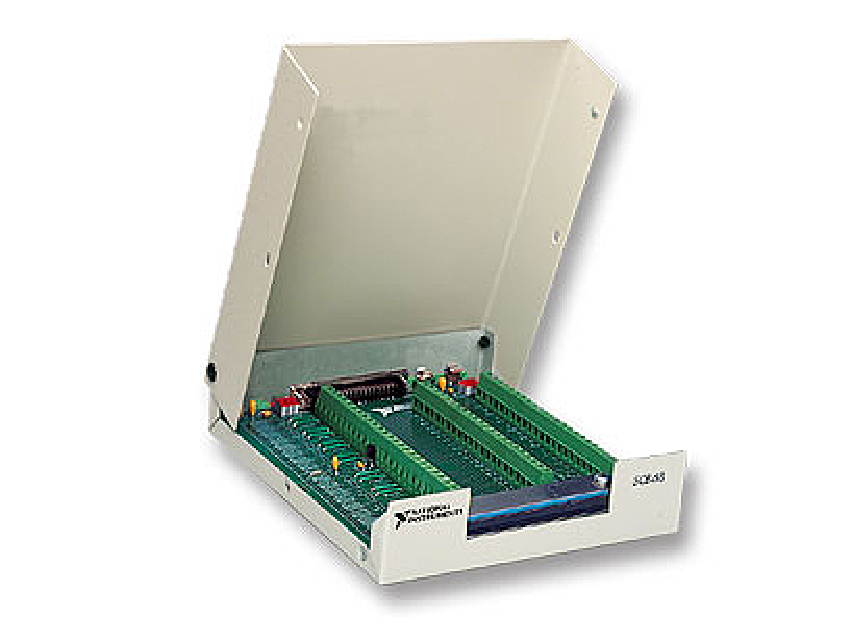
\includegraphics[width=0.7\textwidth]{eps_pics/ioBox}
\caption{NI SCB-60 shielded input/output box that is used for interfacing electrical connections to the 7853R FPGA card. \newline source:www.ni.com
	 \label{fig:ioBox}} 
\end{figure}

\begin{figure}[ht!]
\centering
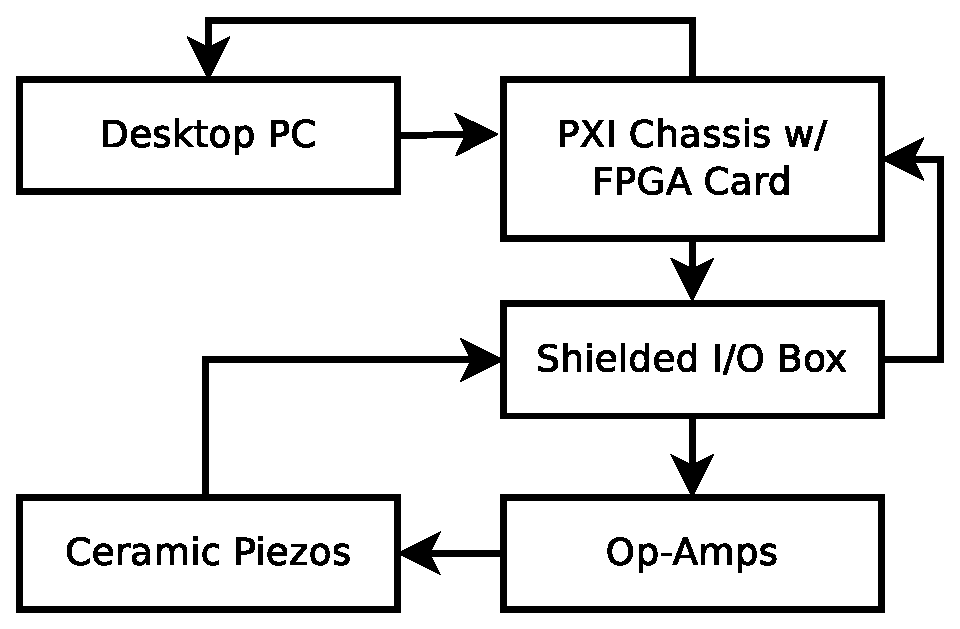
\includegraphics[width=0.7\textwidth]{eps_pics/hardwareComm}
\caption{Diagram which shows the communication hierarchy among the different hardware pieces that were used for testing. The communication between the PC and FPGA card was performed using a MXI cable. The acquisition cables interfaced to the FPGA through an NI shielded I/O box and cable. Any other connections were made using normal insulated copper wire.
	 \label{fig:hardwareComm}} 
\end{figure}

\section{Crack Detection Tests}

The first topic investigated is if the system is able to sense when a defect has become present within the material. This step is important because it would be inefficient and potentially damaging to attempt to perform acoustic focusing when no defect is present in the system.

The setup used for the crack detection involved the use of both nylon and steel solid circular rods. Each rod was approximately $12.7 \times 10^{-3} m$ in diameter. The steel rod was tested first and found to have a density of $7.894 \times 10^3 kg/m^3$, an elastic constant of $169.39 \times 10^9 N/m^2$, and a length of $579 \times 10^{-3} m$. The actuators used to send and receive the signals were piezoceramic stack actuators (PZT) with a diameter of $13 \times 10^{-3} m$ with a piezoelectric strain constant of $d_{33} = 152 \times 10^{-12} C/N$ and a relative permittivity of $\epsilon _{33} = 450 \epsilon _0$ with $\epsilon _0 = 8.854 \times 10 ^{-12} F/m$. Two transducers were affixed to each end of the steel rod using accelerometer putty with PZT A being on the left side of the rod and PZT B being on the right side. This system was then placed into compression using a custom built mechanism. The compression mechanism was created using common nuts and bolts, optics table hardware, and a few machined aluminum blocks (Figure \ref{fig:compression}). The compression could be controlled by the use of a single bolt and was tightened with a small screw driver to one-quarter turn past being finger tight. The experiments were carried out on an optics table which significantly reduced external vibrations through the use of air damping. The setup is shown in Figure \ref{fig:steelUncrackedFull}. Also pictured in the setup is a terminal block that was used for handling the copper wire connections (Figure \ref{fig:junctionBox}). The terminal block also contains a diode circuit consisting of two diodes that is placed between the amplifier output lines and the analog read in lines for each PZT (Figure \ref{fig:diodeCircuit}). The diode circuit snuffs out noise from the amplifier that was found to be large enough to overshadow some test results and will be discussed more in the results section.

\begin{figure}
\begin{subfigmatrix}{2}
\subfigure[Left side compression mechanism]
{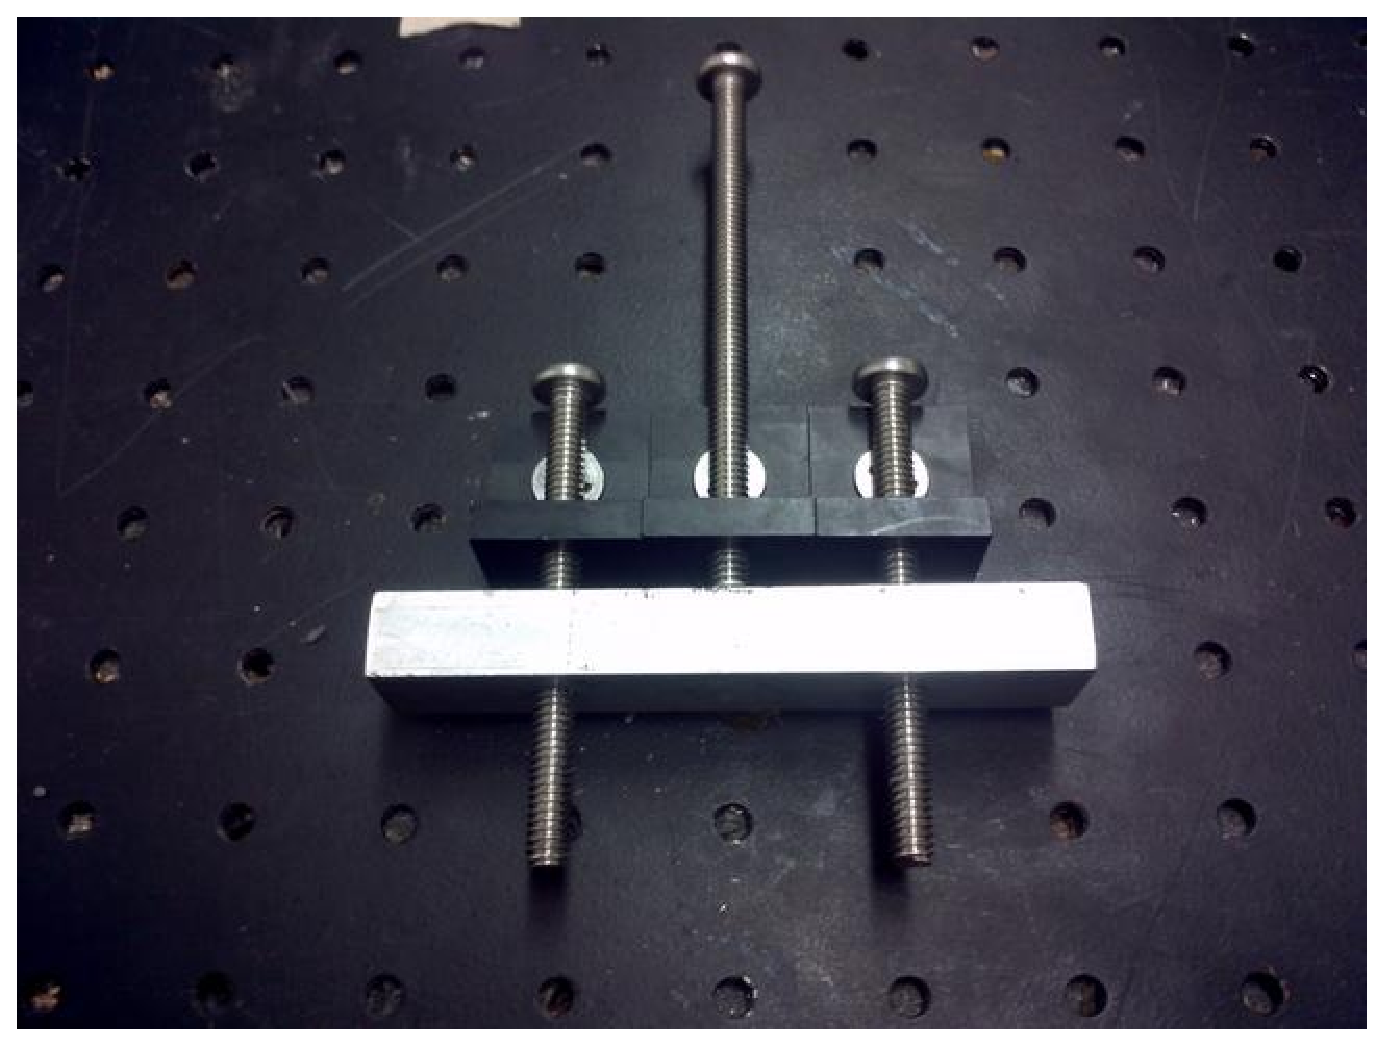
\includegraphics[width=0.7\textwidth]{eps_pics/lsCompression}}
\subfigure[Right side compression mechanism ]
{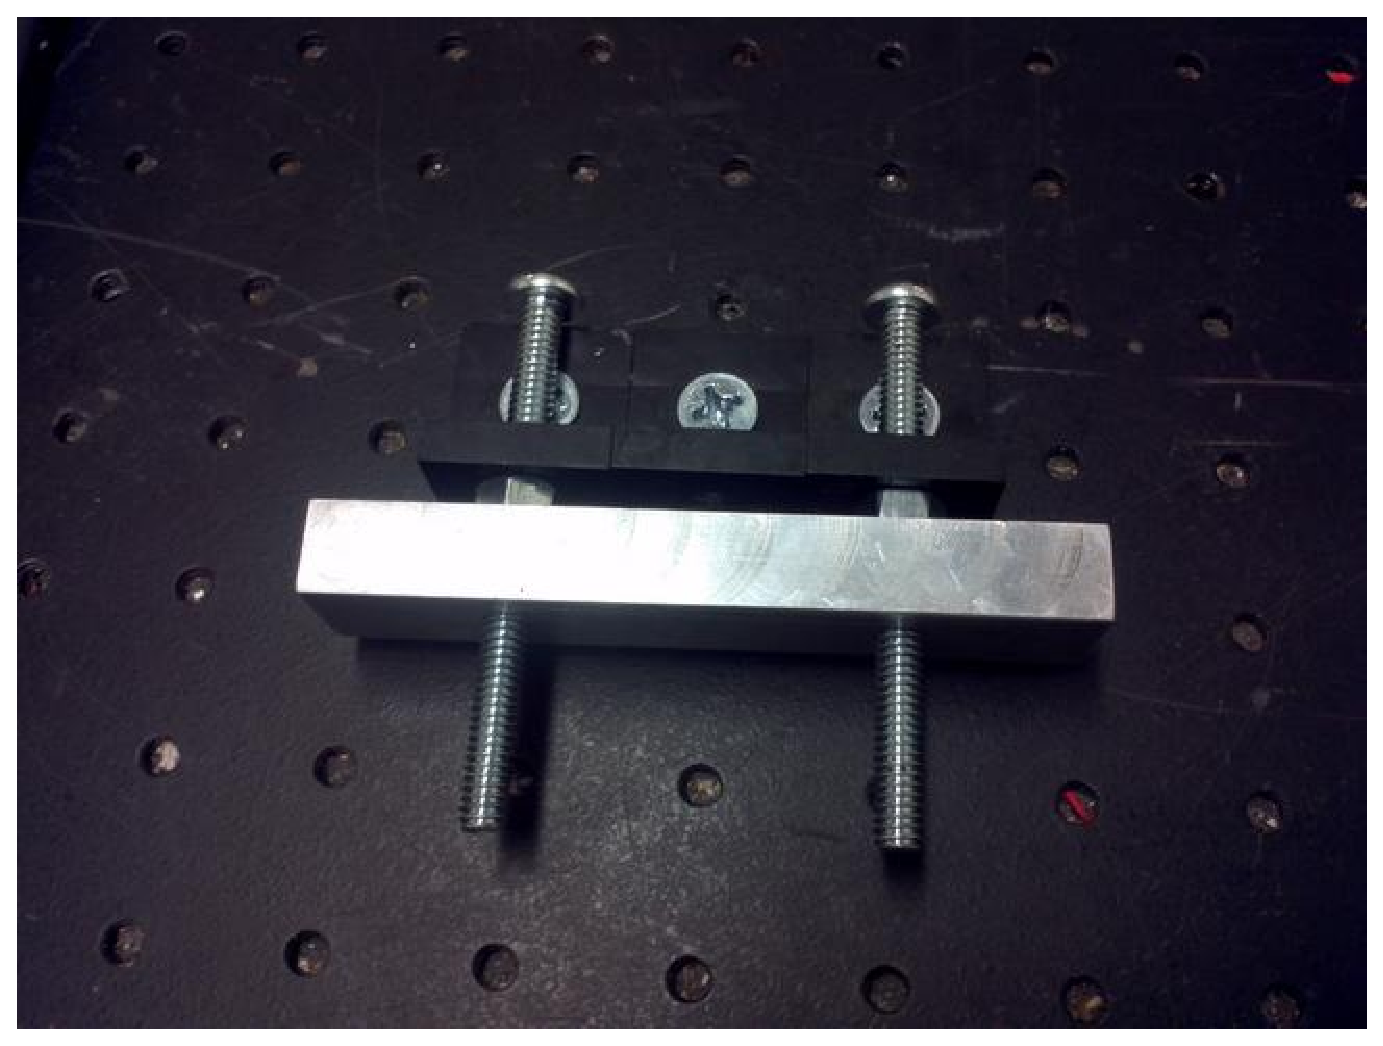
\includegraphics[width=0.7\textwidth]{eps_pics/rsCompression}}
\end{subfigmatrix}

   \caption[all]
%>>>> use \label inside caption to get Fig. number with \ref{}
   { \label{fig:compression}
(a) The left side compression mechanism. The middle bolt was used to adjust the compression in the system by using it to move the aluminum block back and forth;
(b) Right side compression mechanism. This had two nuts to adjust the aluminum bar's positions so it could accommodate different rod sizes.
 }
   \end{figure}

\begin{figure}[ht!]
\centering
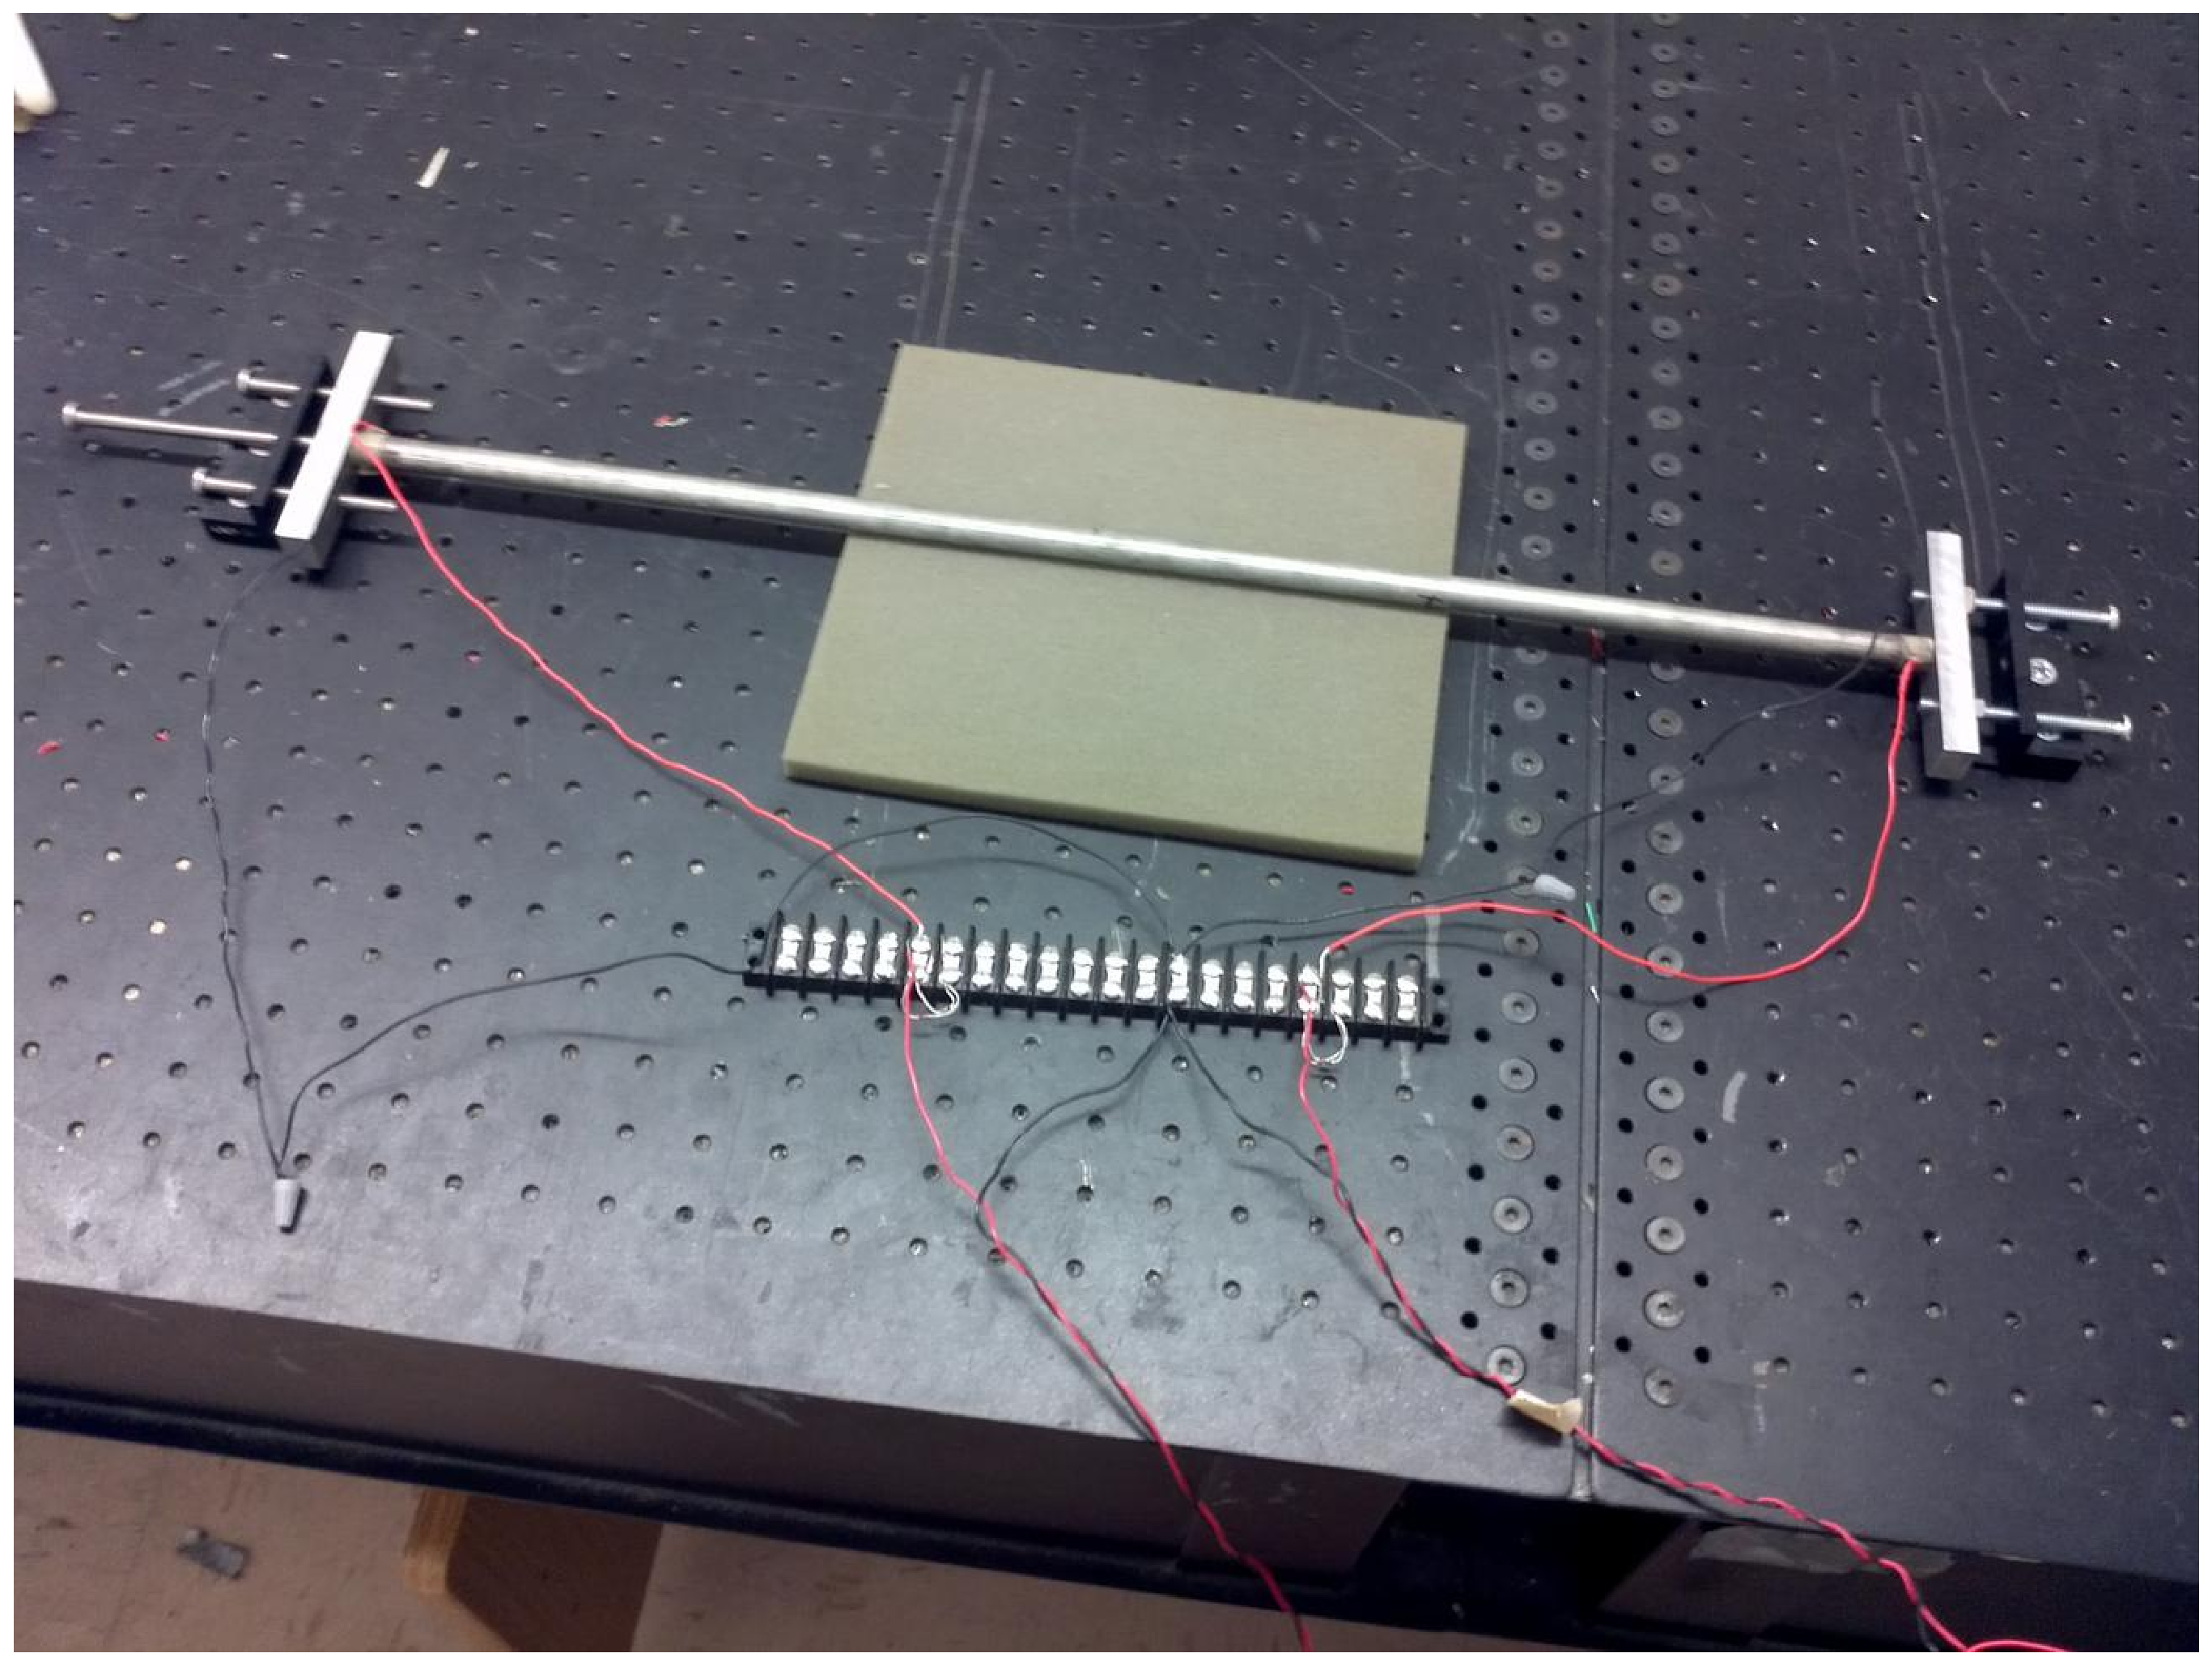
\includegraphics[width=0.7\textwidth]{eps_pics/steelUncrackedFull}
\caption{Steel rod with PZTs affixed to each end using accelerometer putty. The system is in compression using the custom mechanism and is seen on the optics table. The PZT on the left is referred to as PZT A and the right PZT is referred to as PZT B. 
 	 \label{fig:steelUncrackedFull}} 
\end{figure}

\begin{figure}[ht!]
\centering
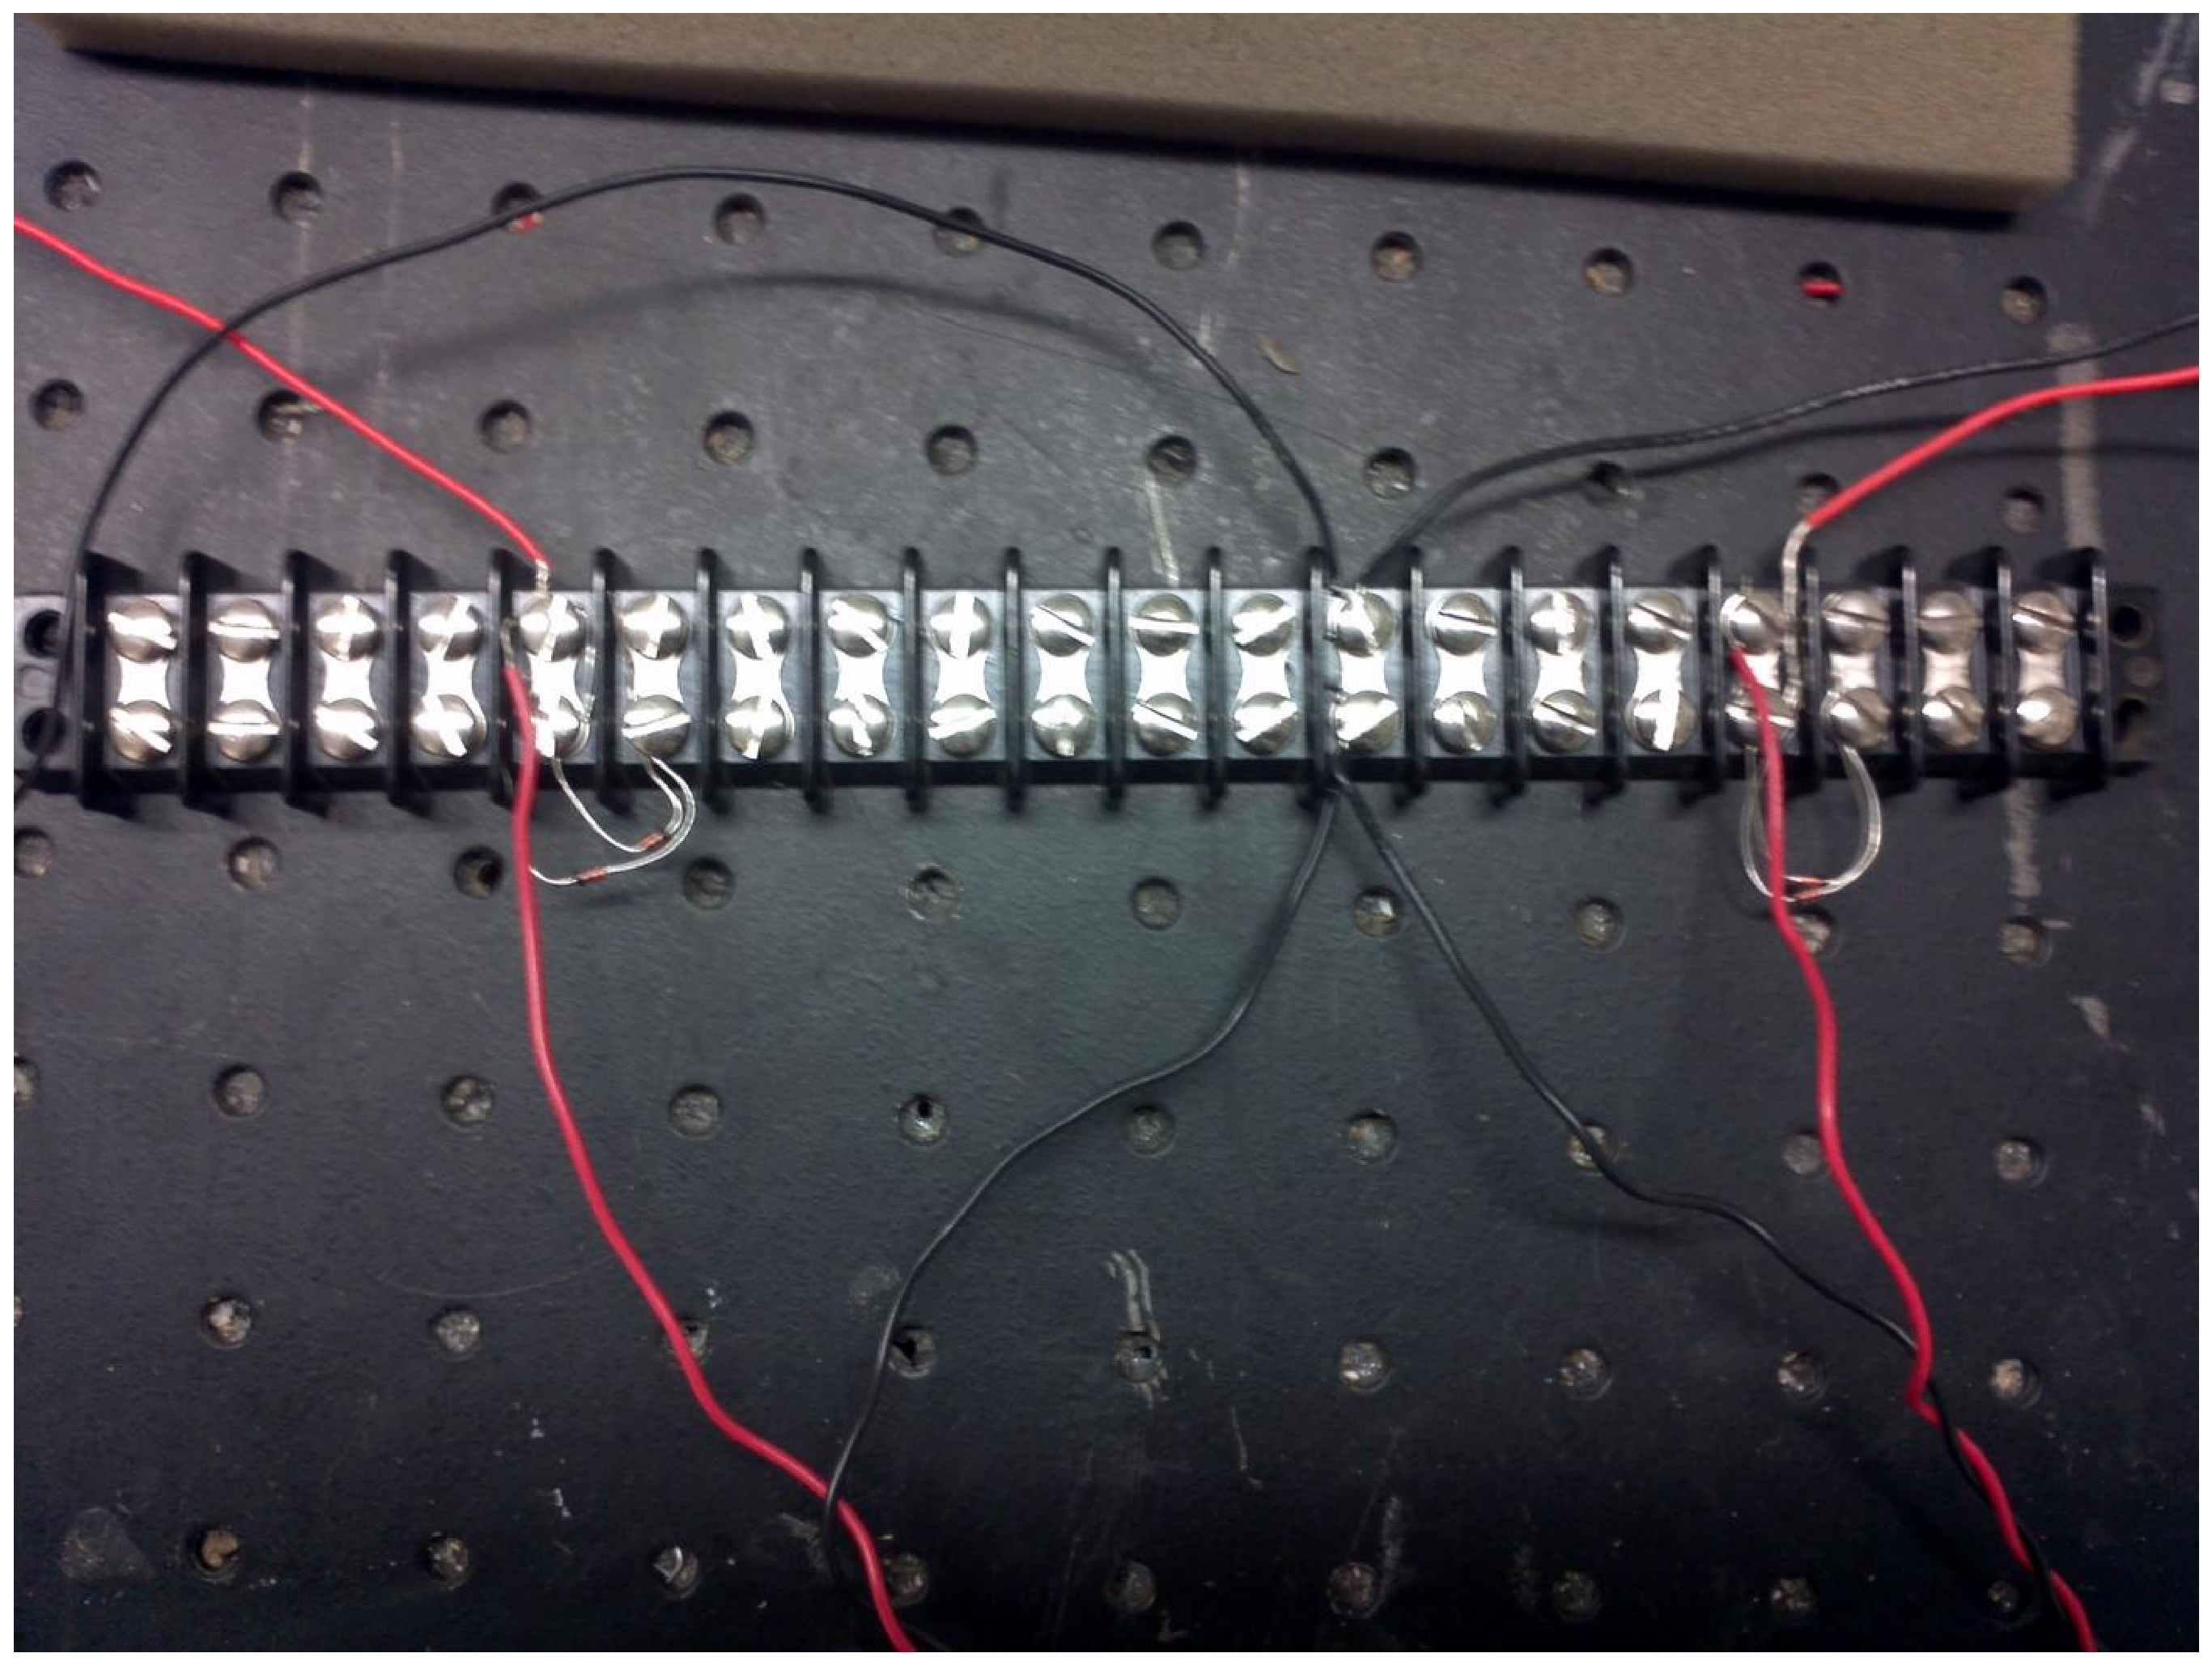
\includegraphics[width=0.7\textwidth]{eps_pics/junctionBox}
\caption{Simple terminal block that was used for handling the connections among the various data acquisition wires. Also contained on the terminal block is a diode circuit between the amplifier output and the analog read in line for each PZT. 
 	 \label{fig:junctionBox}} 
\end{figure}

\begin{figure}[ht!]
\centering
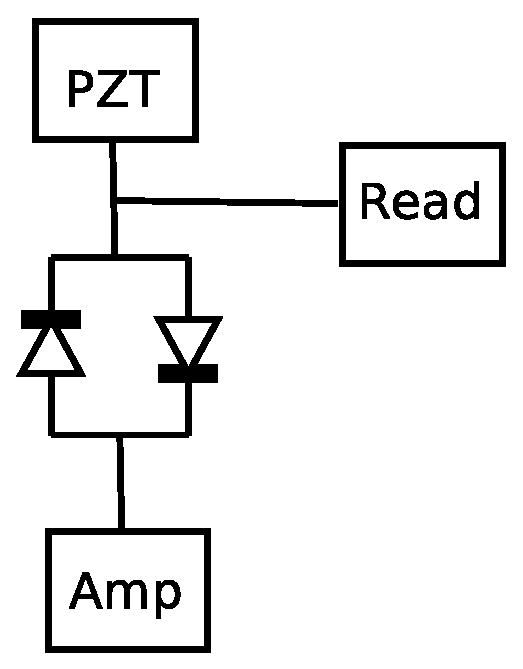
\includegraphics[width=0.3\textwidth]{eps_pics/diodeCircuit}
\caption{Diode circuit that is placed between the amplifier output and analog read in lines for each PZT. This circuit snuffs out the noise produced by the amplifiers at the expense of a slight reduction in voltage output to the PZTs. 
 	 \label{fig:diodeCircuit}} 
\end{figure}

The software used consisted of two main programs which were the host program and the FPGA program. The host program ran on the PC and the FPGA program was downloaded to the FPGA card where it was executed. Communication between the host and FPGA programs was handled with the FPGA's First-In-First-Out memory protocol (FIFO) to which the host program had direct memory access (DMA).The synchronization of the data transactions between the host and FPGA programs is handles using a handshaking protocol implemented by IRQs. 

The purpose of this set of experiments was to determine if the occurrence of a crack could be detected within the steel rod. The idea is to send a signal from PZT A and record the response at PZT B. This continues and successive responses are compared to the first response and the program attempts to detect a significant change between the responses which indicates that something in the medium has changed and potentially represents the appearance of a crack. For the implementation, the host program first generated an initial multi-tone wave. The wave is composed of individual sinusoidal waves of different frequency that were concatenated together to form the overall mutli-tone wave. The center frequency for the multi-tone wave was $115 kHz$ and had a bandwidth of $30 kHz$. The relationship between the number of points needed to create the wave and the sampling frequency of the FPGA card (740.741 kHz here) was used to obtain the correct frequency for each wave. A total of 7,8, and 9 data points were used by the program to represent a single sinusoidal wave period of the $130 kHz$, $115 kHz$, and $100 kHz$ wave components, respectively. The $130kHz$ wave was placed in the center of the wave grouping with a $115kHz$ wave on both sides of it and then a $100 kHz$ wave on the ends of the grouping (Figure \ref{fig:initialWave}). 

\begin{figure}[ht!]
\centering
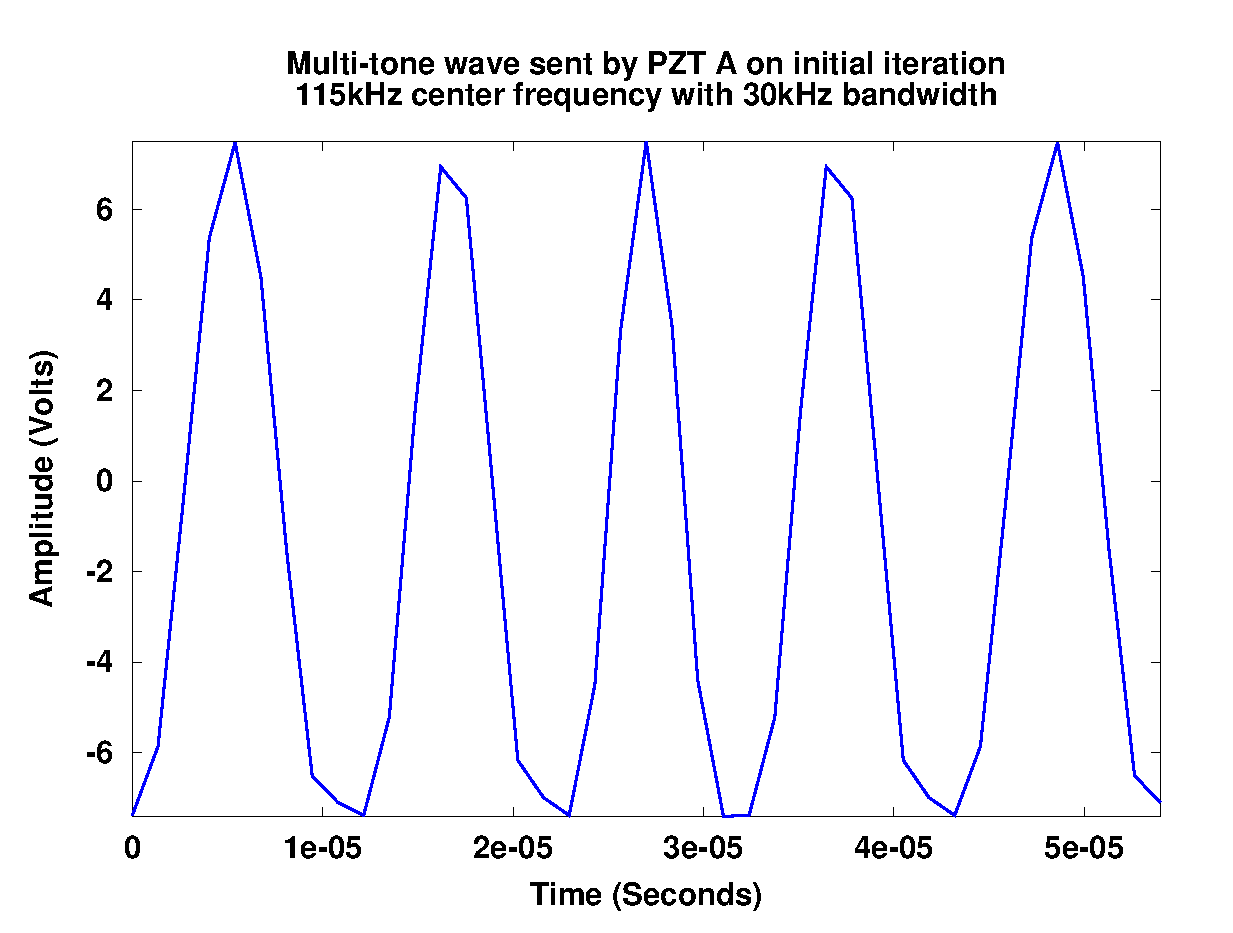
\includegraphics[width=0.6\textwidth]{eps_pics/initialWave}
\caption{Mutli-tone wave that was played out by PZT A. The wave was created by concatenating single period sinusoidal waves of different frequency. The wave in the middle is $130kHz$, the waves next to it are $115kHz$, and the outside waves are $100kHz$. It was found that this multi-tone wave caused a better response in the material versus using a single frequency.
 	 \label{fig:initialWave}} 
\end{figure}

After the wave was generated it was transferred to the FPGA program which then zeroed all of its output values and waited for $200ms$. This wait time was chosen based upon experimental results for the time of a signal to decay when propagating through a steel or nylon rod. Once the wait time elapsed, the signal was sent into the rod by PZT A. The wave propagated through the rod and was recorded on the other end by PZT B. This was performed five times total and the response for each iteration was recorded. With the data for the undamaged rod recorded it was time to test a damaged sample. The damaged steel rod was created  by taking the undamaged rod that was used and cutting it in to two pieces of arbitrary length (Figure \ref{fig:steelPieces}). A PZT was placed on one end of each piece and the free ends of the pieces were pressed together. What was formed was essentially the same rod that was previously but with a crack location at an arbitrary position (Figure \ref{fig:steelCrack}). The program was then ran five times on the new setup with a signal being sent by PZT A and recorded at PZT B.

\begin{figure}[ht!]
\centering
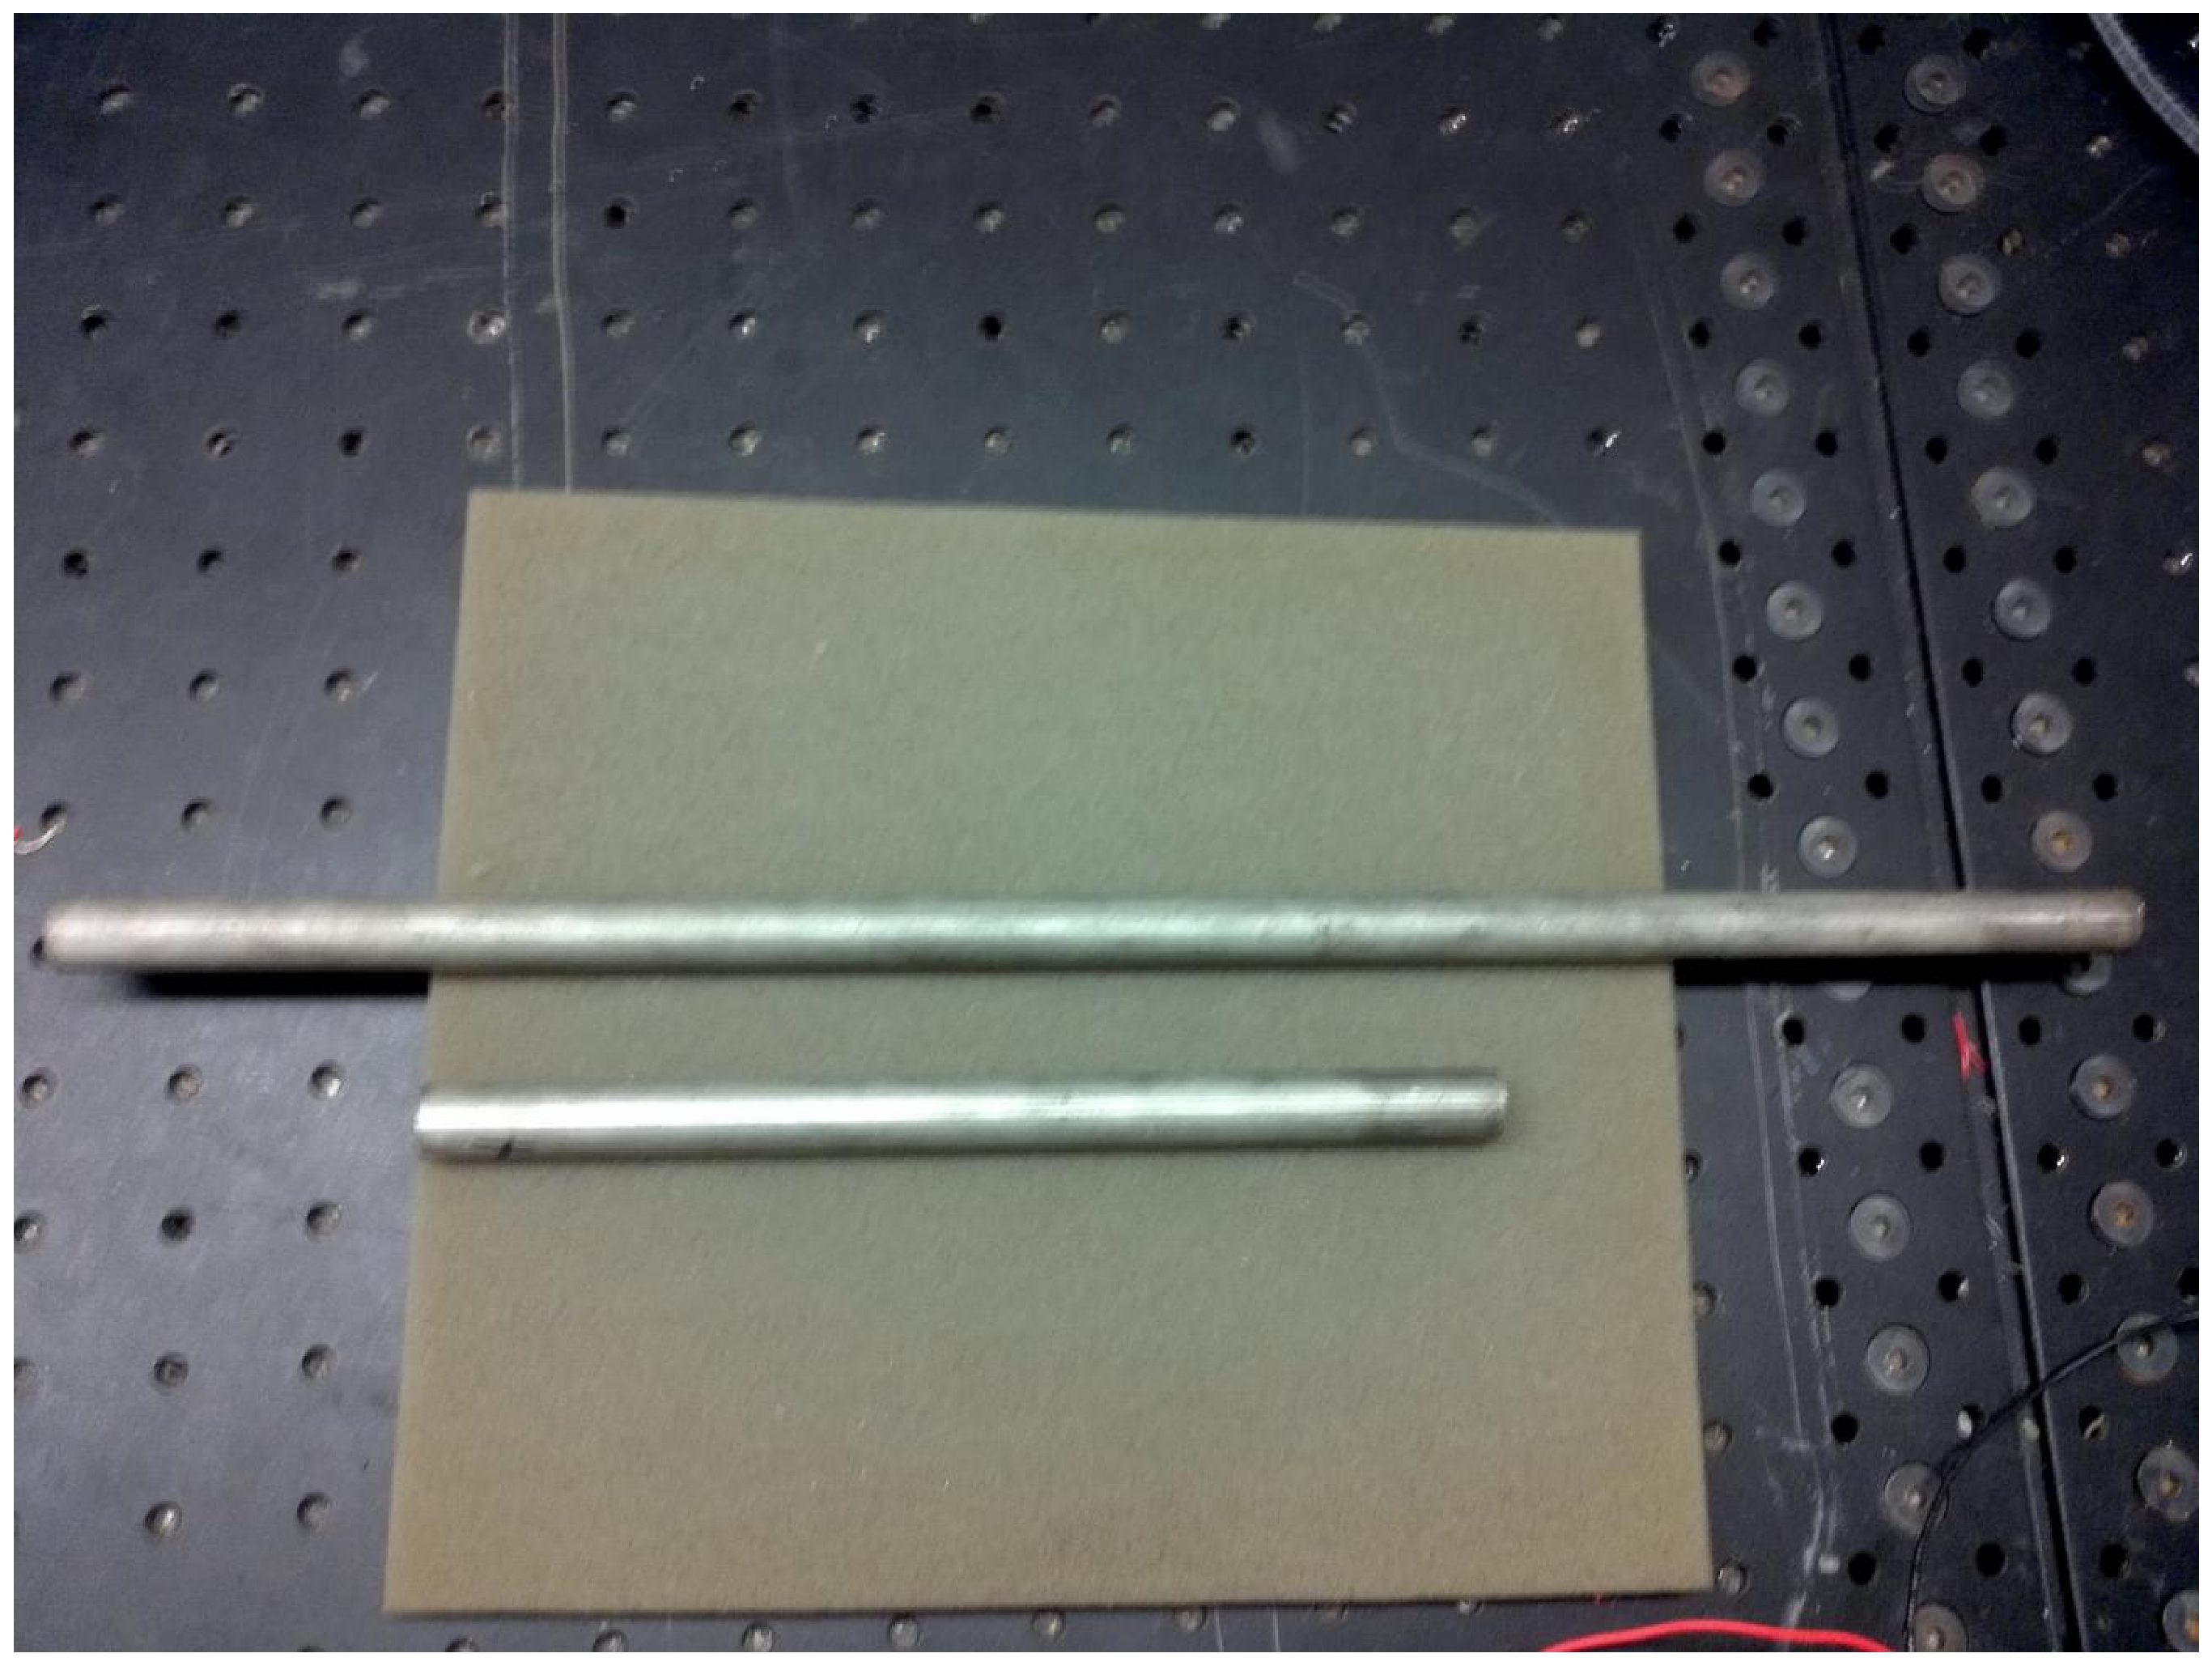
\includegraphics[width=0.6\textwidth]{eps_pics/steelPieces}
\caption{Undamaged rod that has been cut in to two pieces of random length. This pieces are then pushed together (end to end) to represent a rod with a crack location.
 	 \label{fig:steelPieces}} 
\end{figure}

\begin{figure}
\begin{subfigmatrix}{2}
\subfigure[Full view of steel 'damaged rod' tests]
{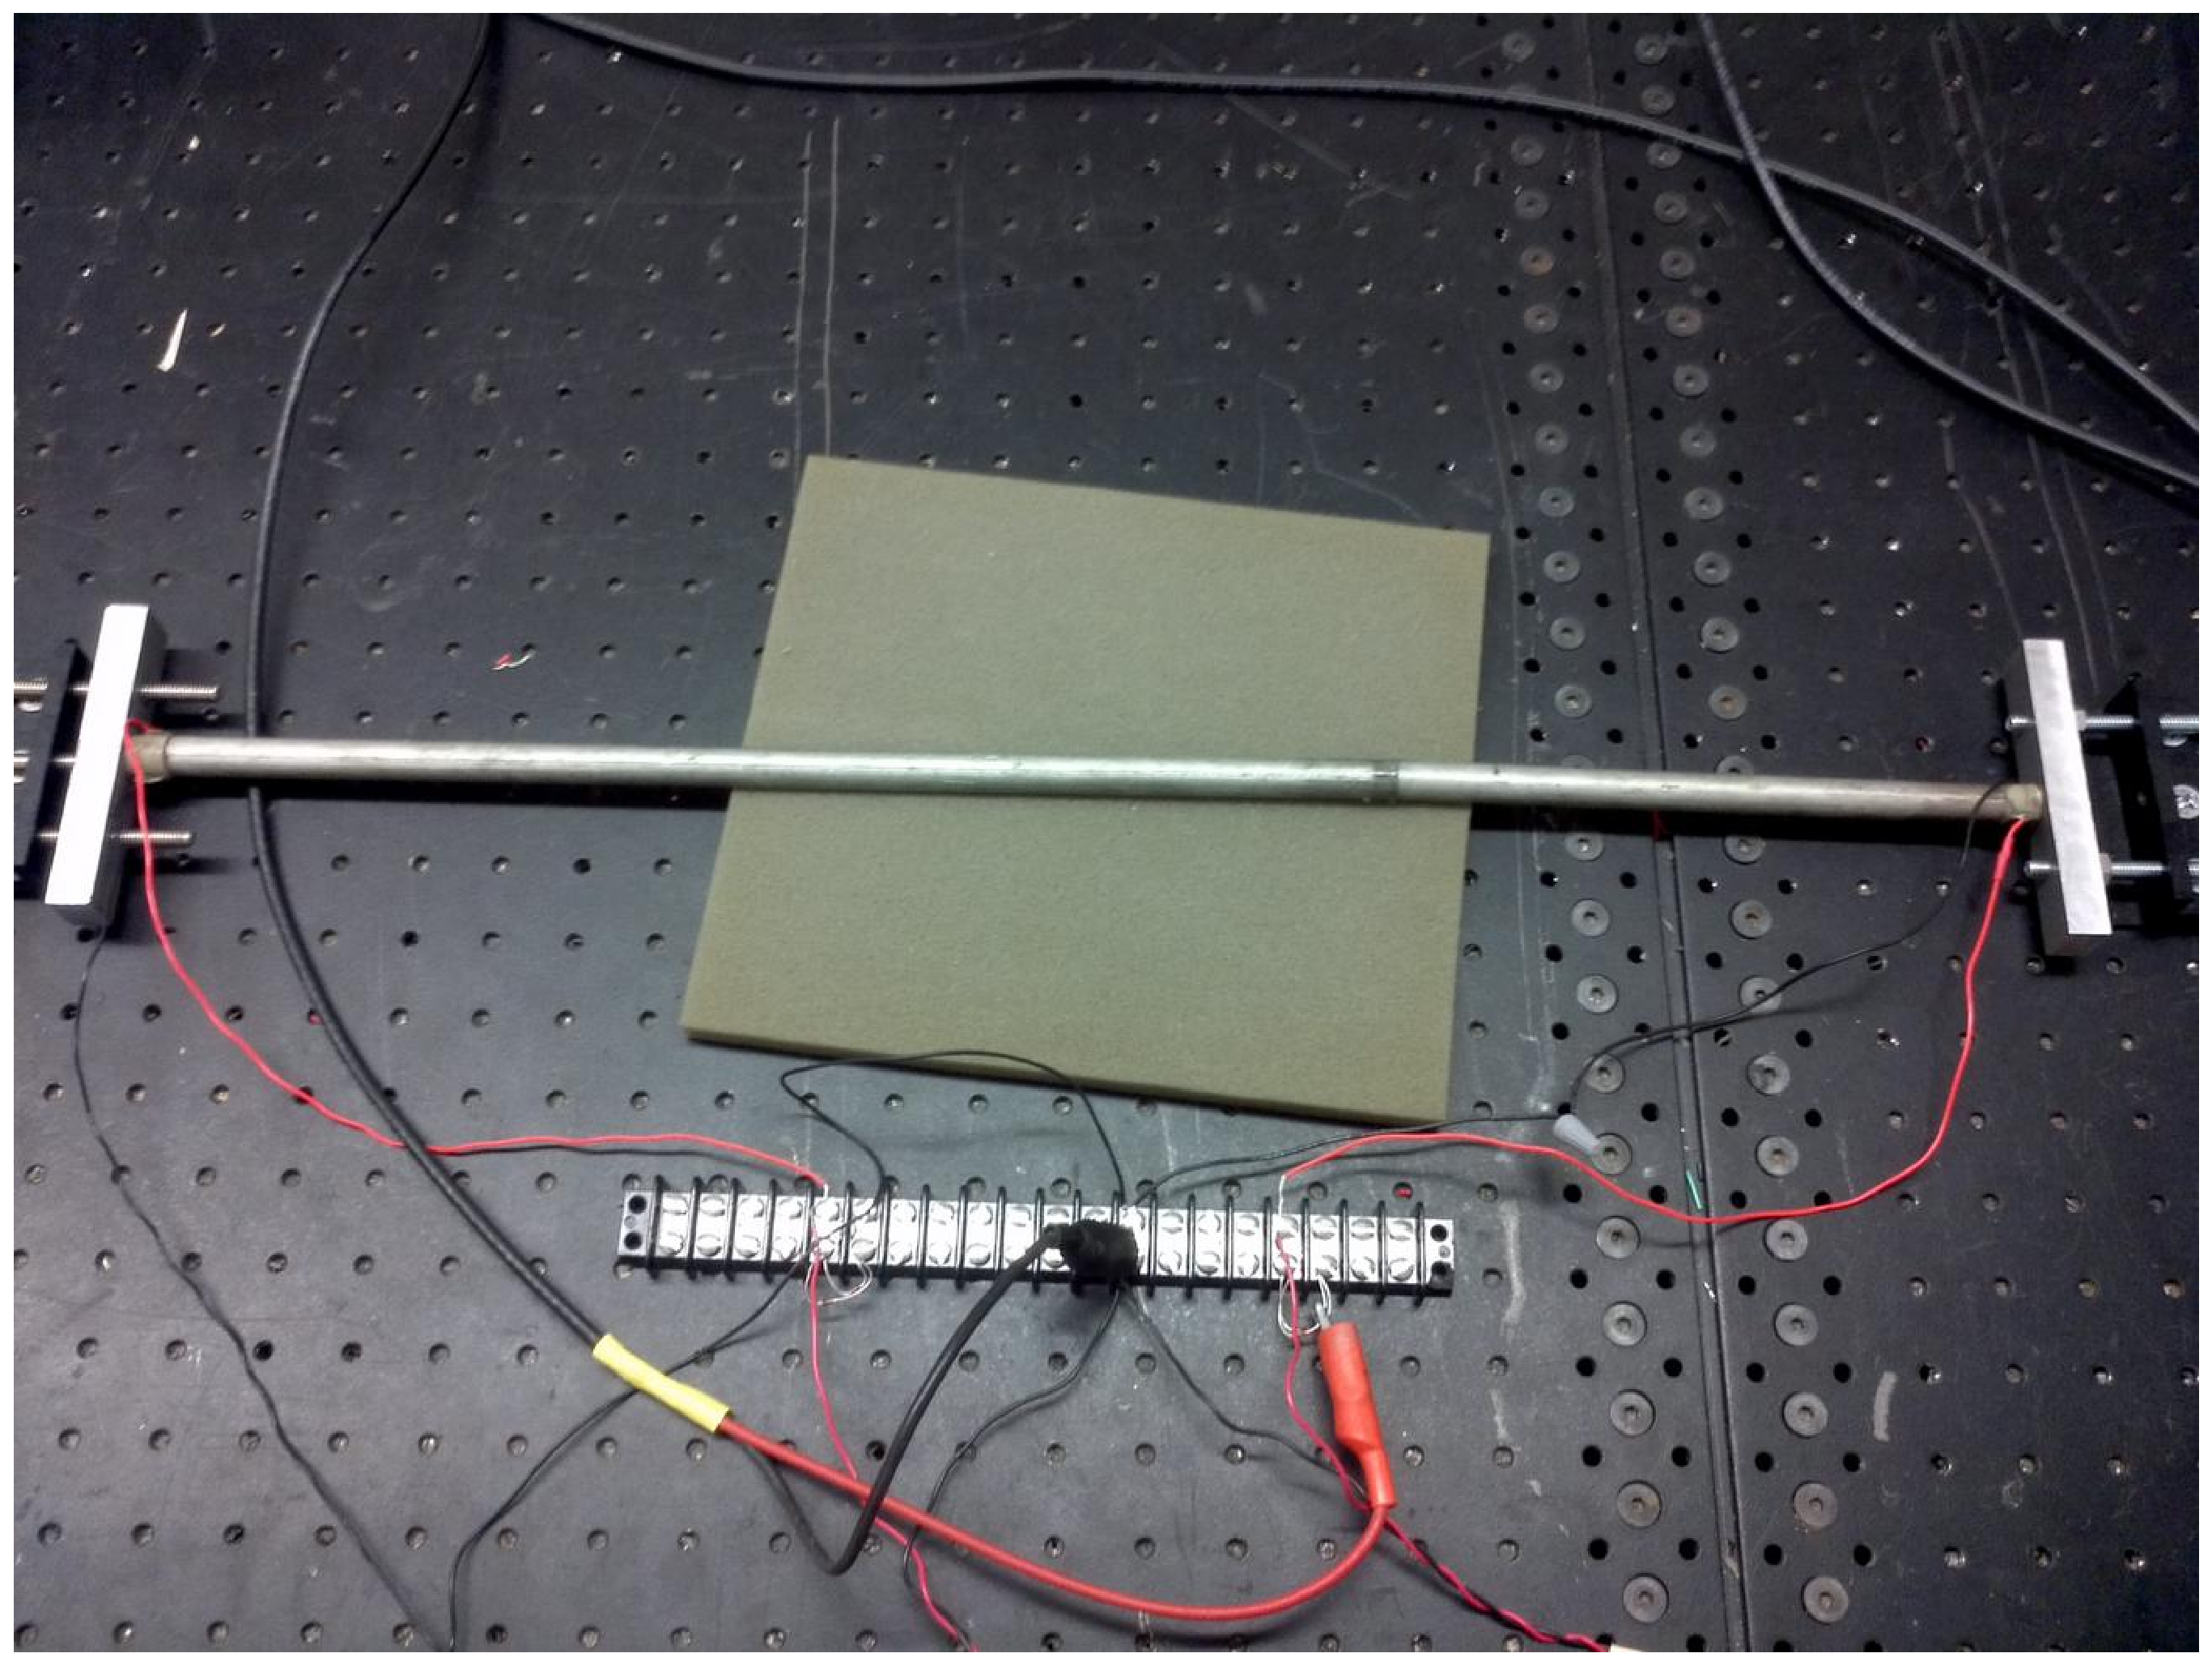
\includegraphics[width=0.6\textwidth]{eps_pics/steelCrackFull}}
\subfigure[Close up of the defect location ]
{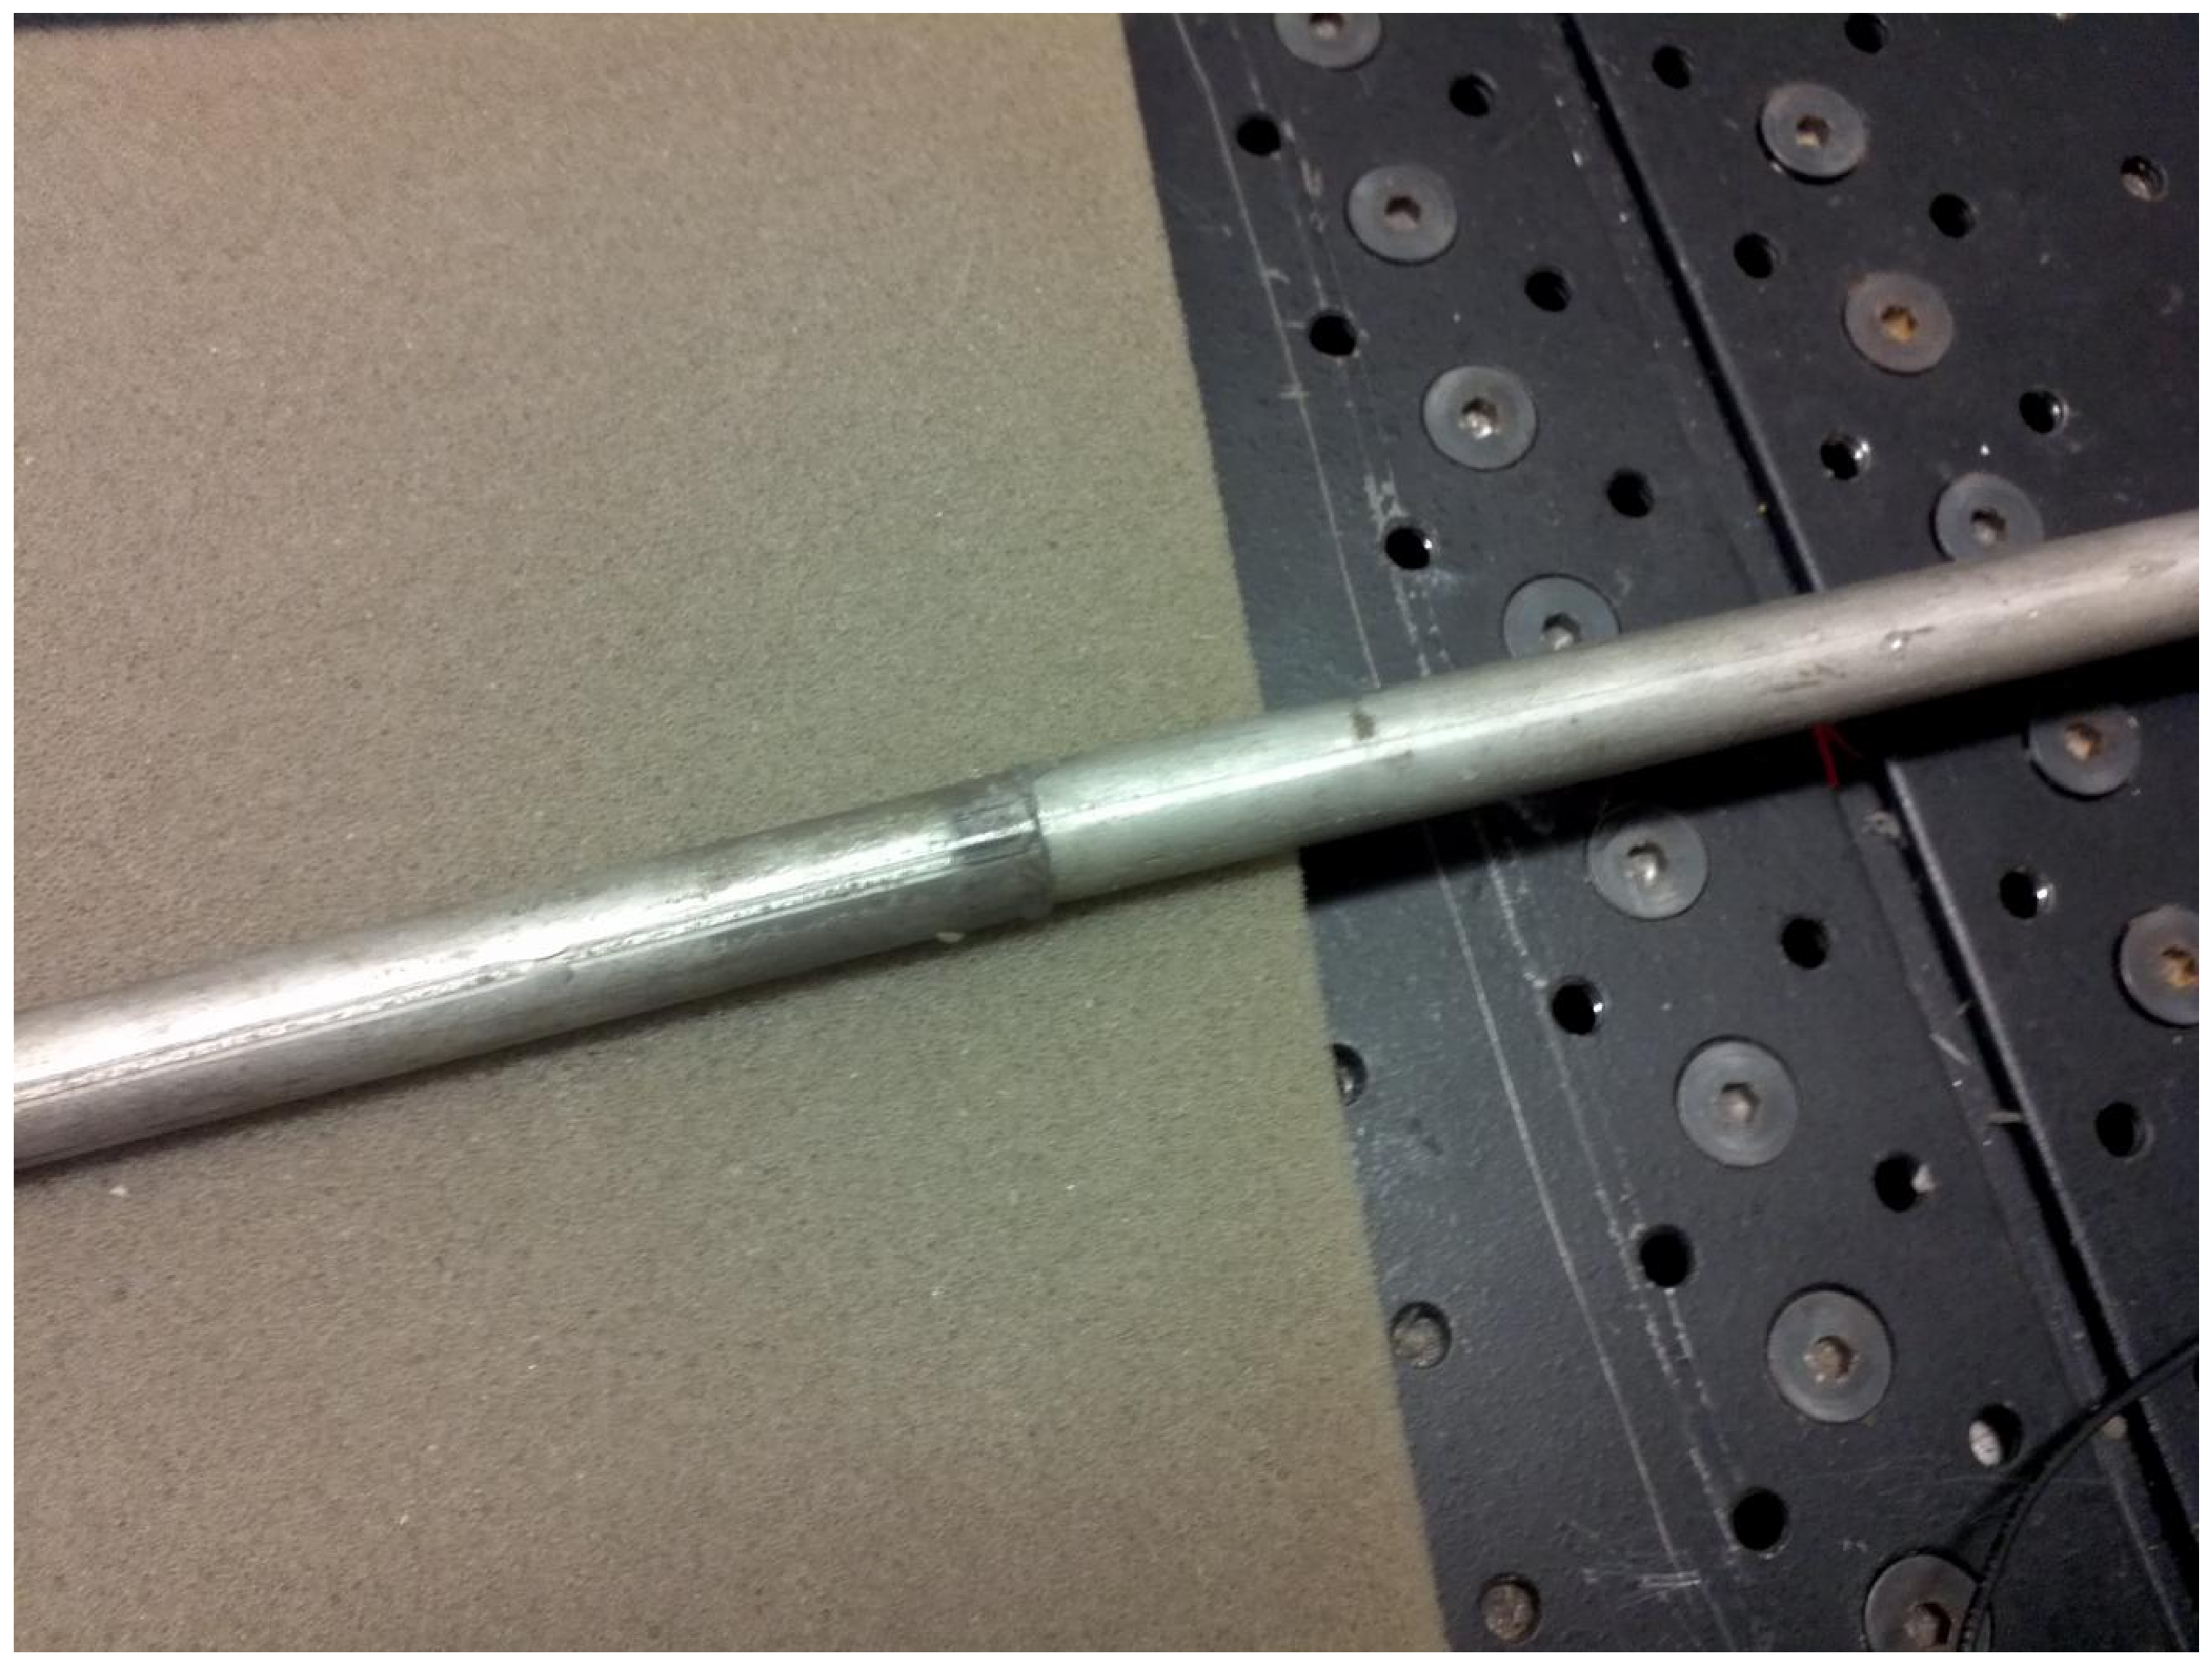
\includegraphics[width=0.6\textwidth]{eps_pics/steelCrackClose}}
\end{subfigmatrix}

   \caption[all]
%>>>> use \label inside caption to get Fig. number with \ref{}
   { \label{fig:steelCrack}
(a) Full view of the two steel rod pieces that are pressed together to represent a rod with a defect location.;
(b) Close up view of the defect location in the steel rod system which should cause a noticeable change in the response at PZT B.
 }
   \end{figure}
   
A MATLAB program read in the data from each run and compared the responses using a simple sum of differences squared formula. The five signals for each test were also averaged together to get a better idea of what the signal looks like in the undamaged tests compared to the damaged rod tests.

These exact same tests were then carried out for a nylon rod. The nylon rod was found to have a density of $0.854 \times 10^3 kg/m^3$, an elastic constant of $4.68121 \times 10^9$ and a length of $148 \times 10^{-3} m$. The setup for the nylon rod tests is shown in Figures \ref{fig:nylonUncrackedFull} and \ref{fig:nylonCrack}.


\begin{figure}[ht!]
\centering
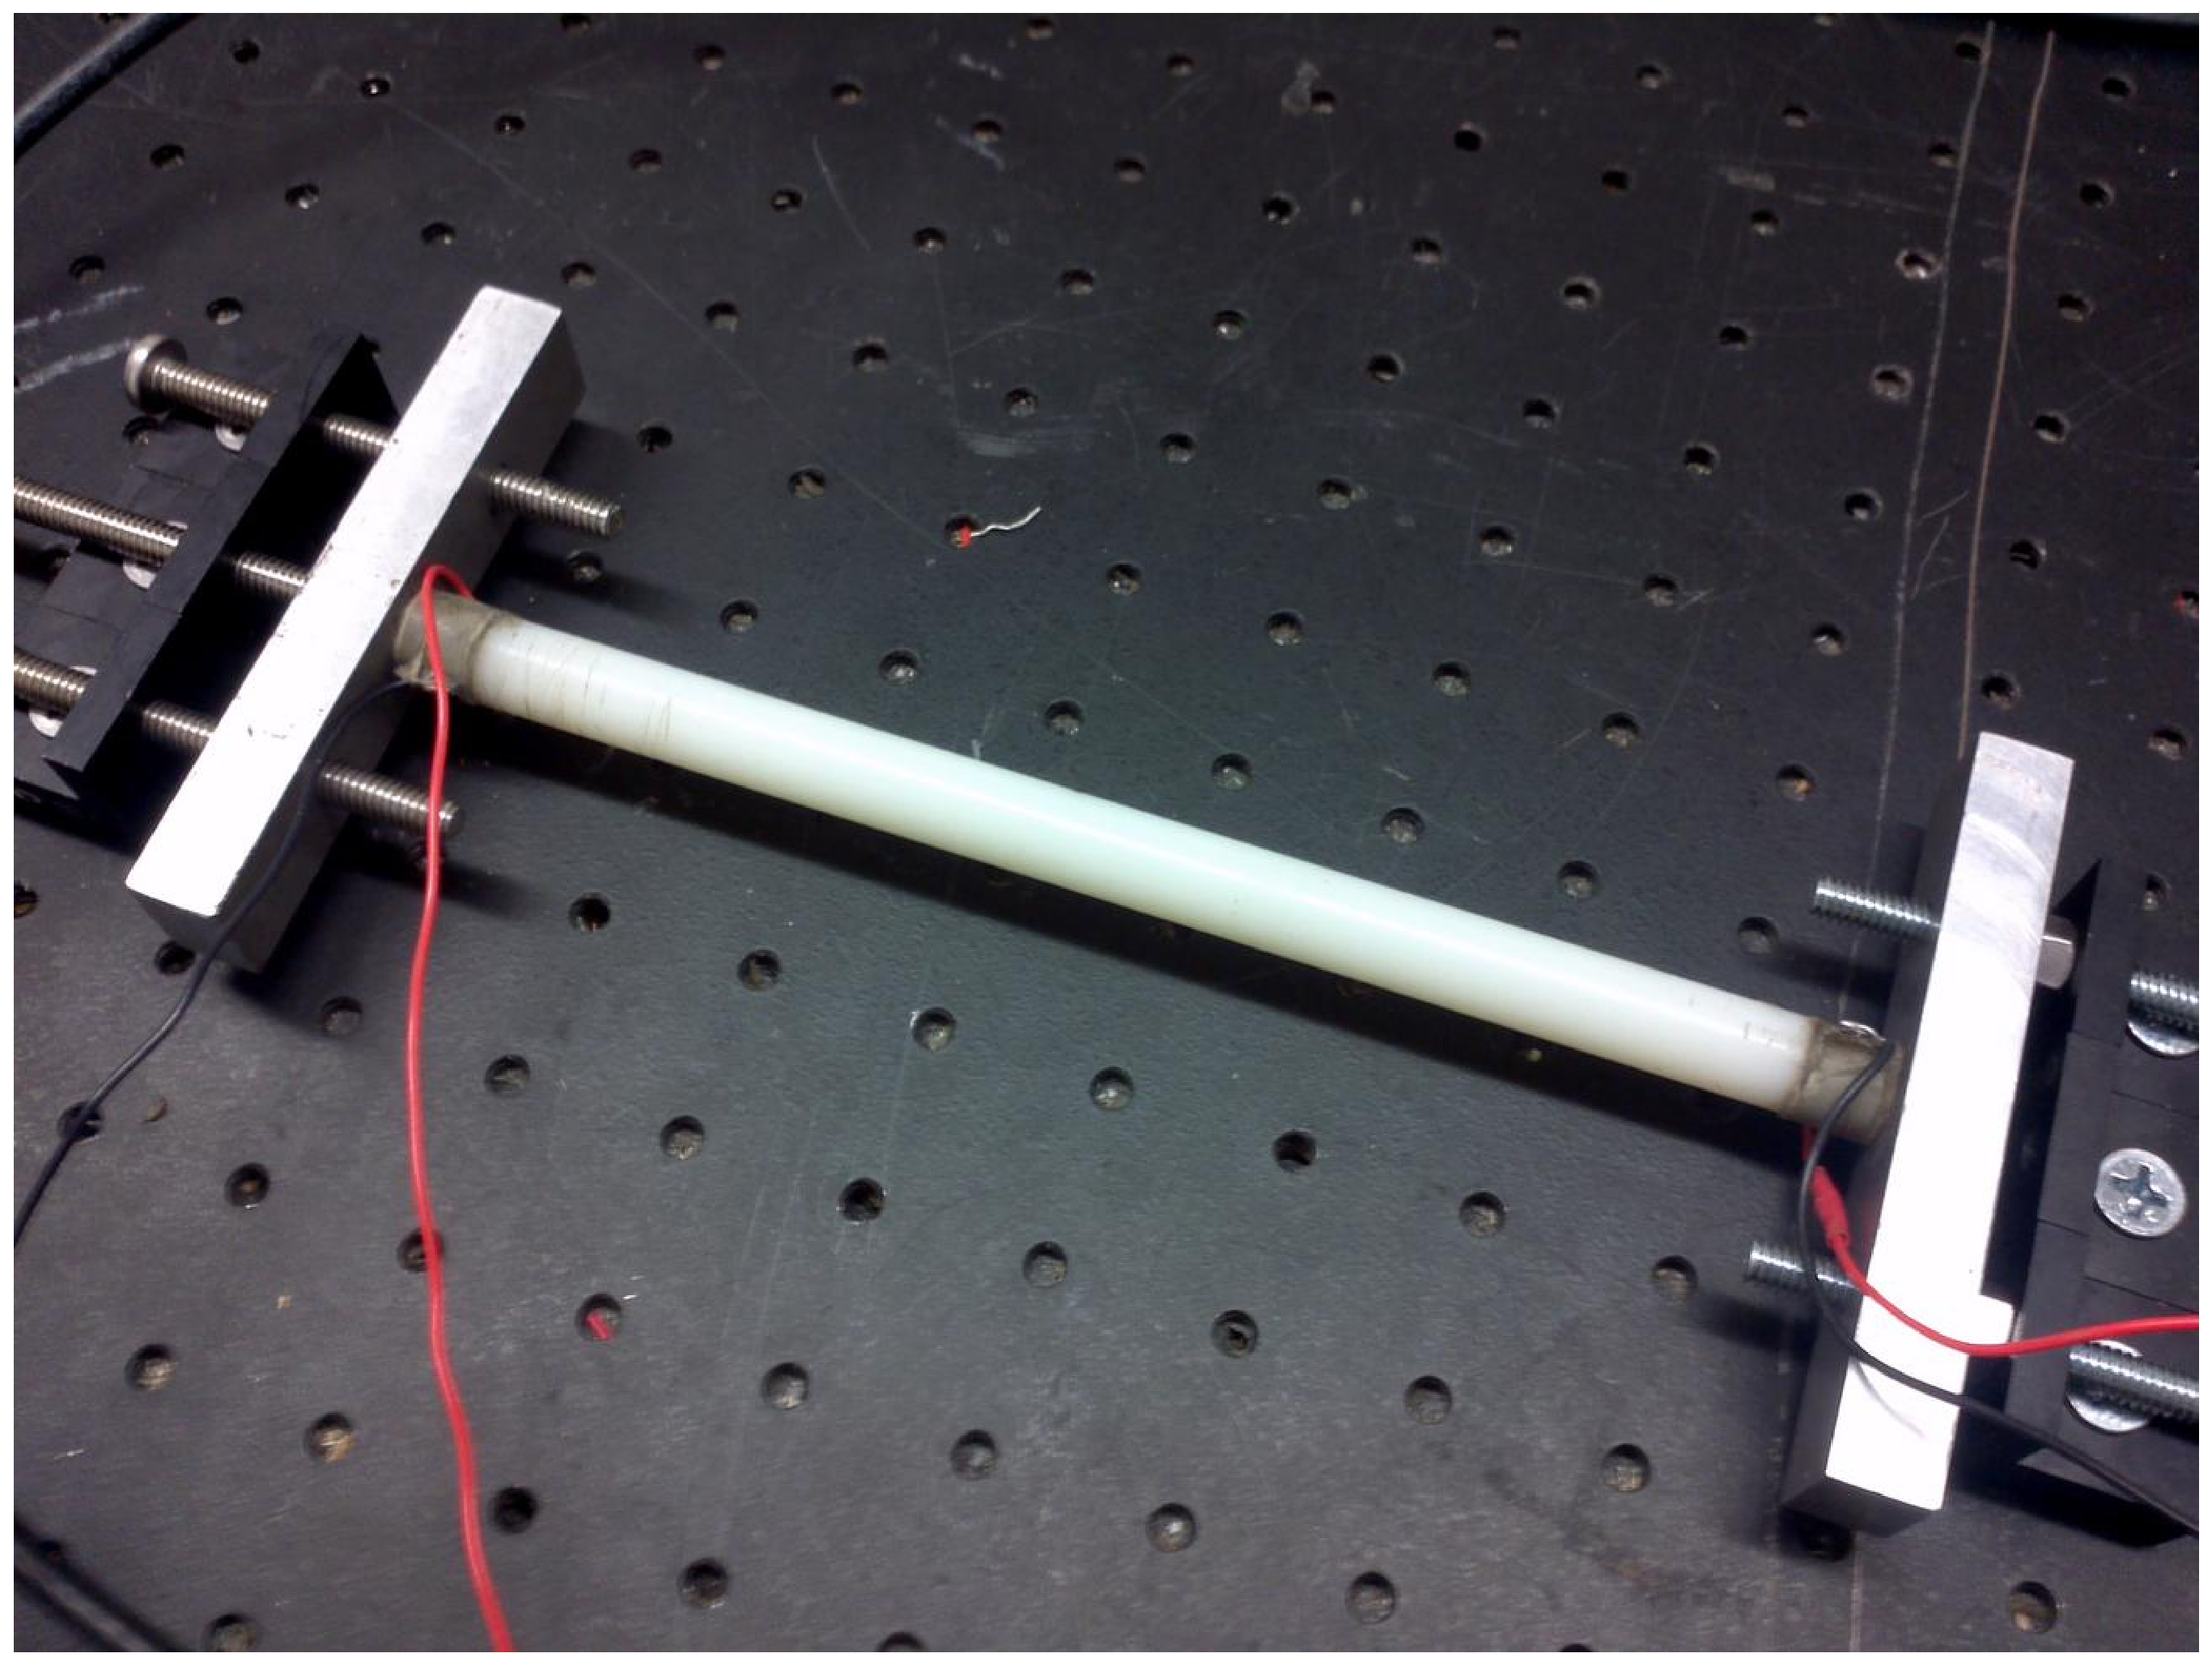
\includegraphics[width=0.6\textwidth]{eps_pics/nylonUncrackedFull}
\caption{Undamaged nylon rod that is setup for testing. A PZT was affixed to each rod end using accelerometer putty and placed into compression using the custom mechanism.
 	 \label{fig:nylonUncrackedFull}} 
\end{figure}

\begin{figure}
\begin{subfigmatrix}{2}
\subfigure[Full view of nylon 'damaged rod' tests]
{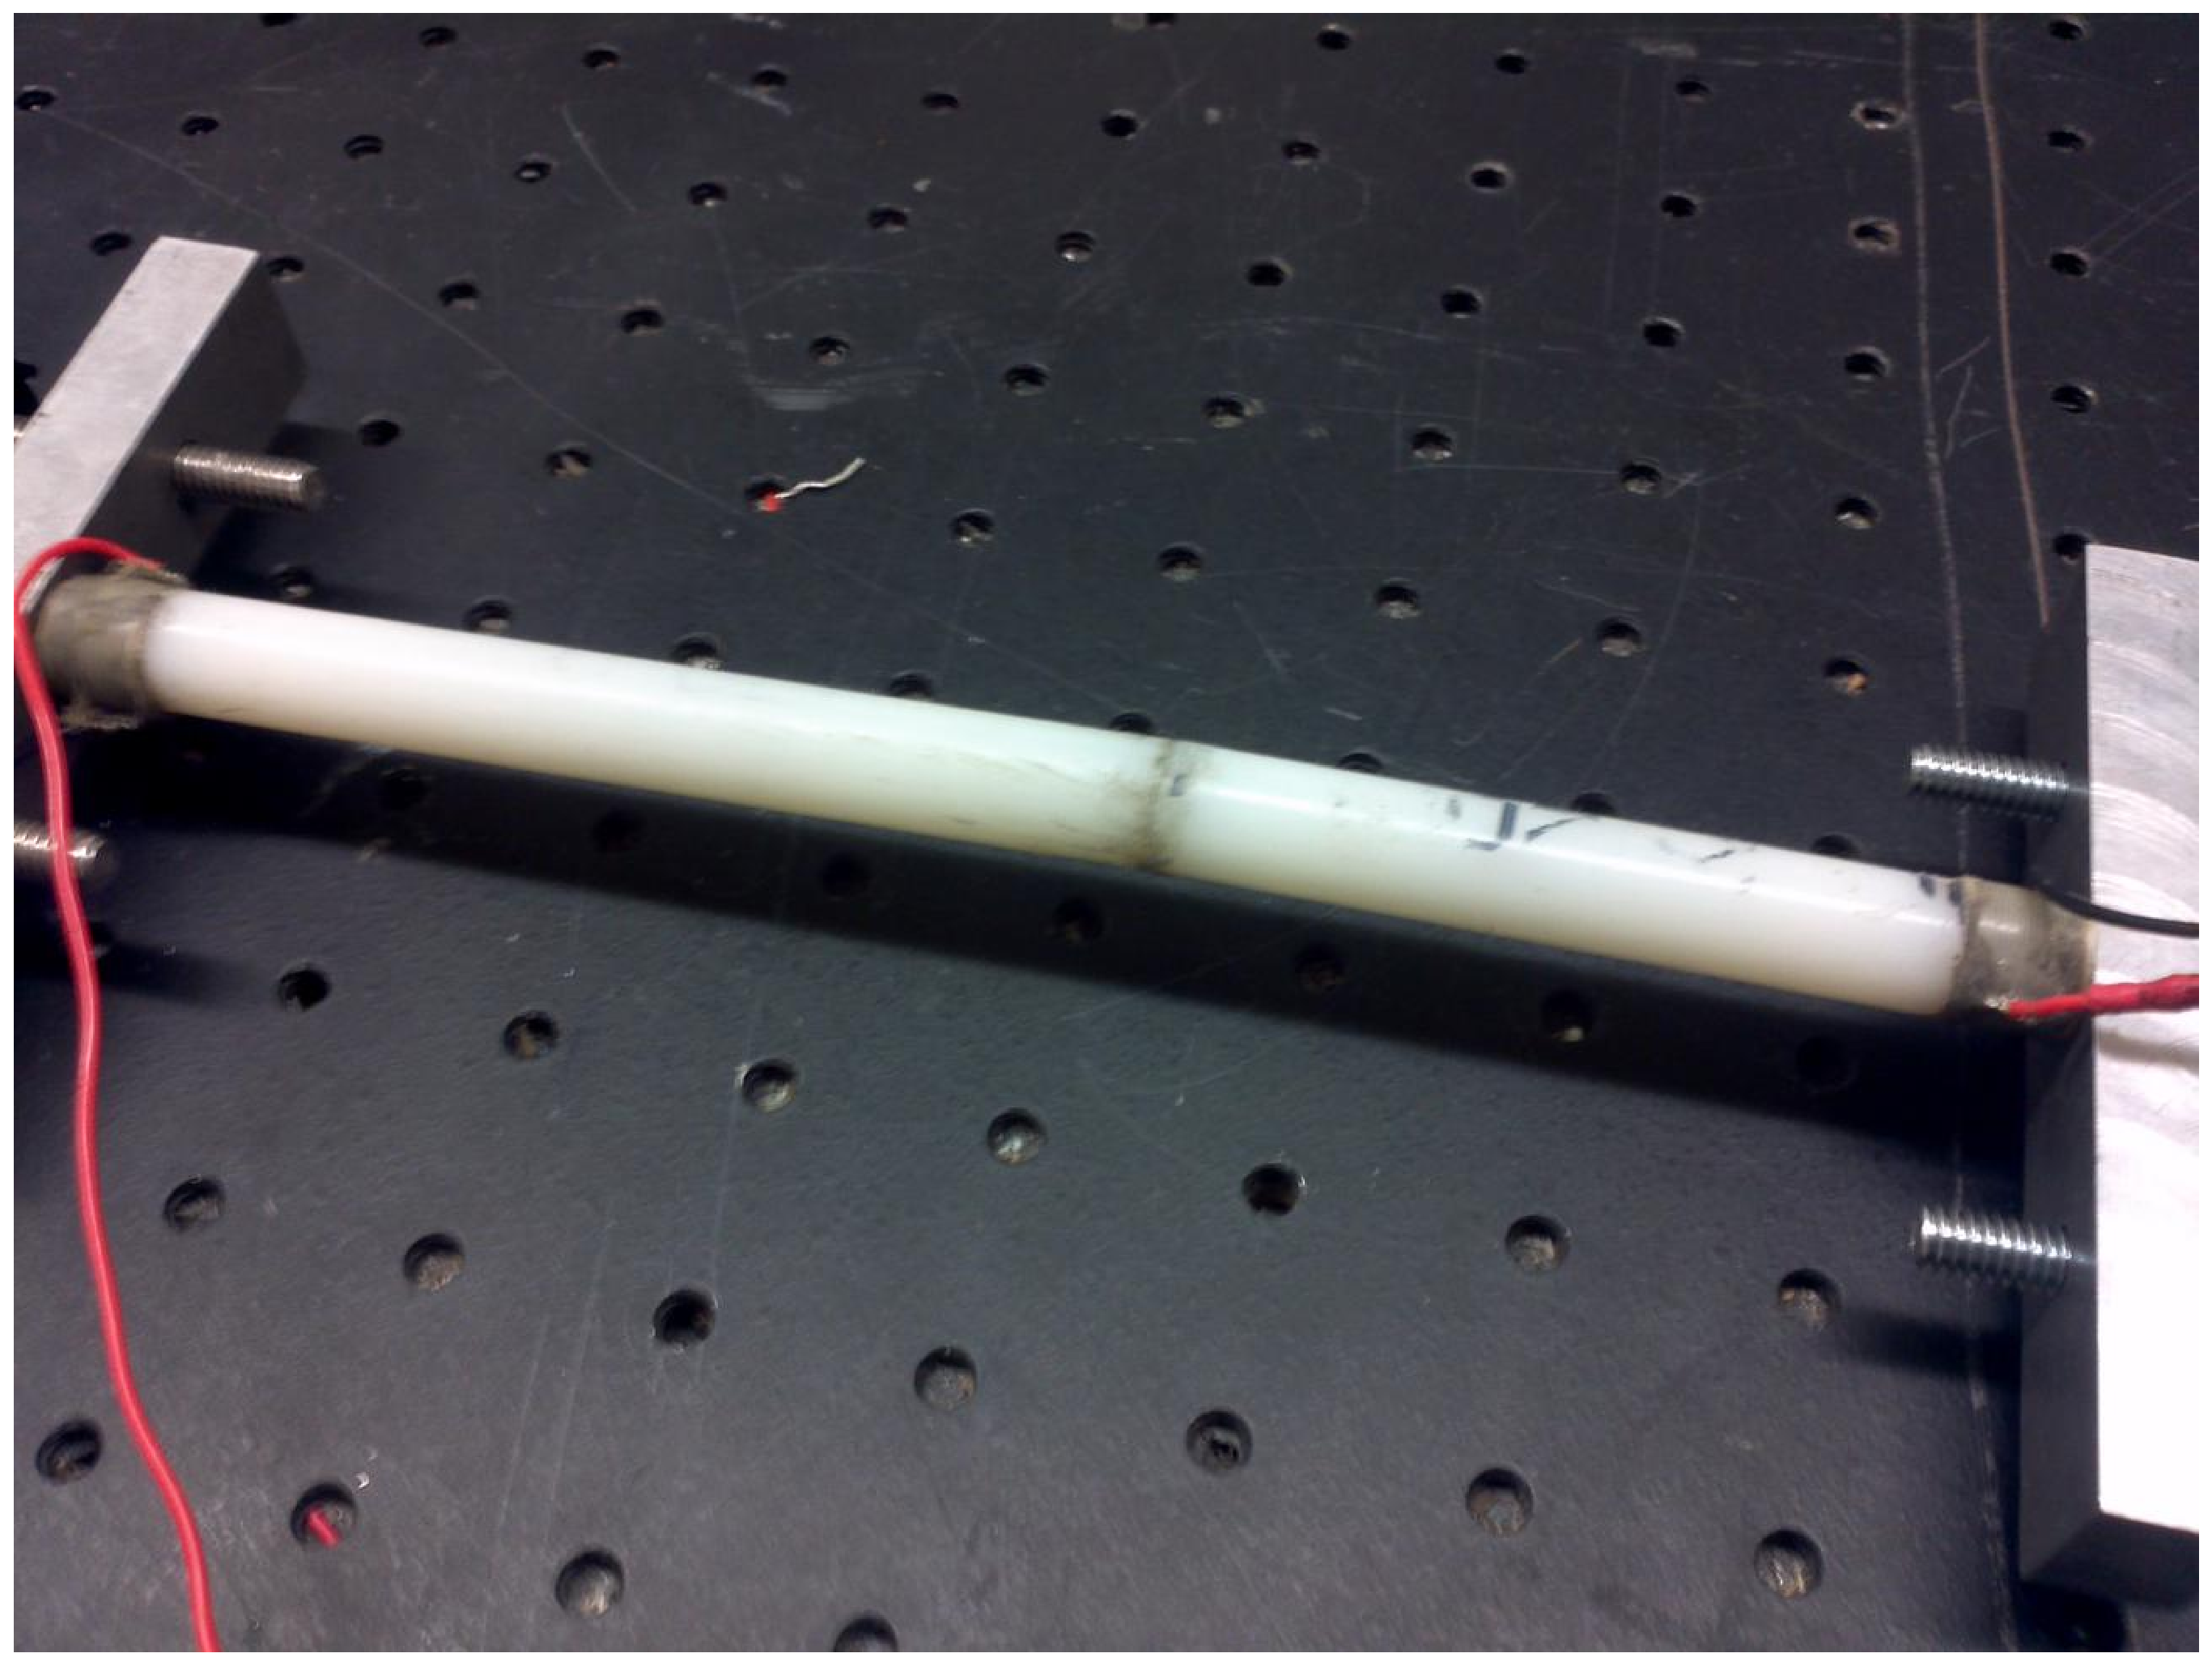
\includegraphics[width=0.6\textwidth]{eps_pics/nylonCrackFull}}
\subfigure[Close up of the defect location ]
{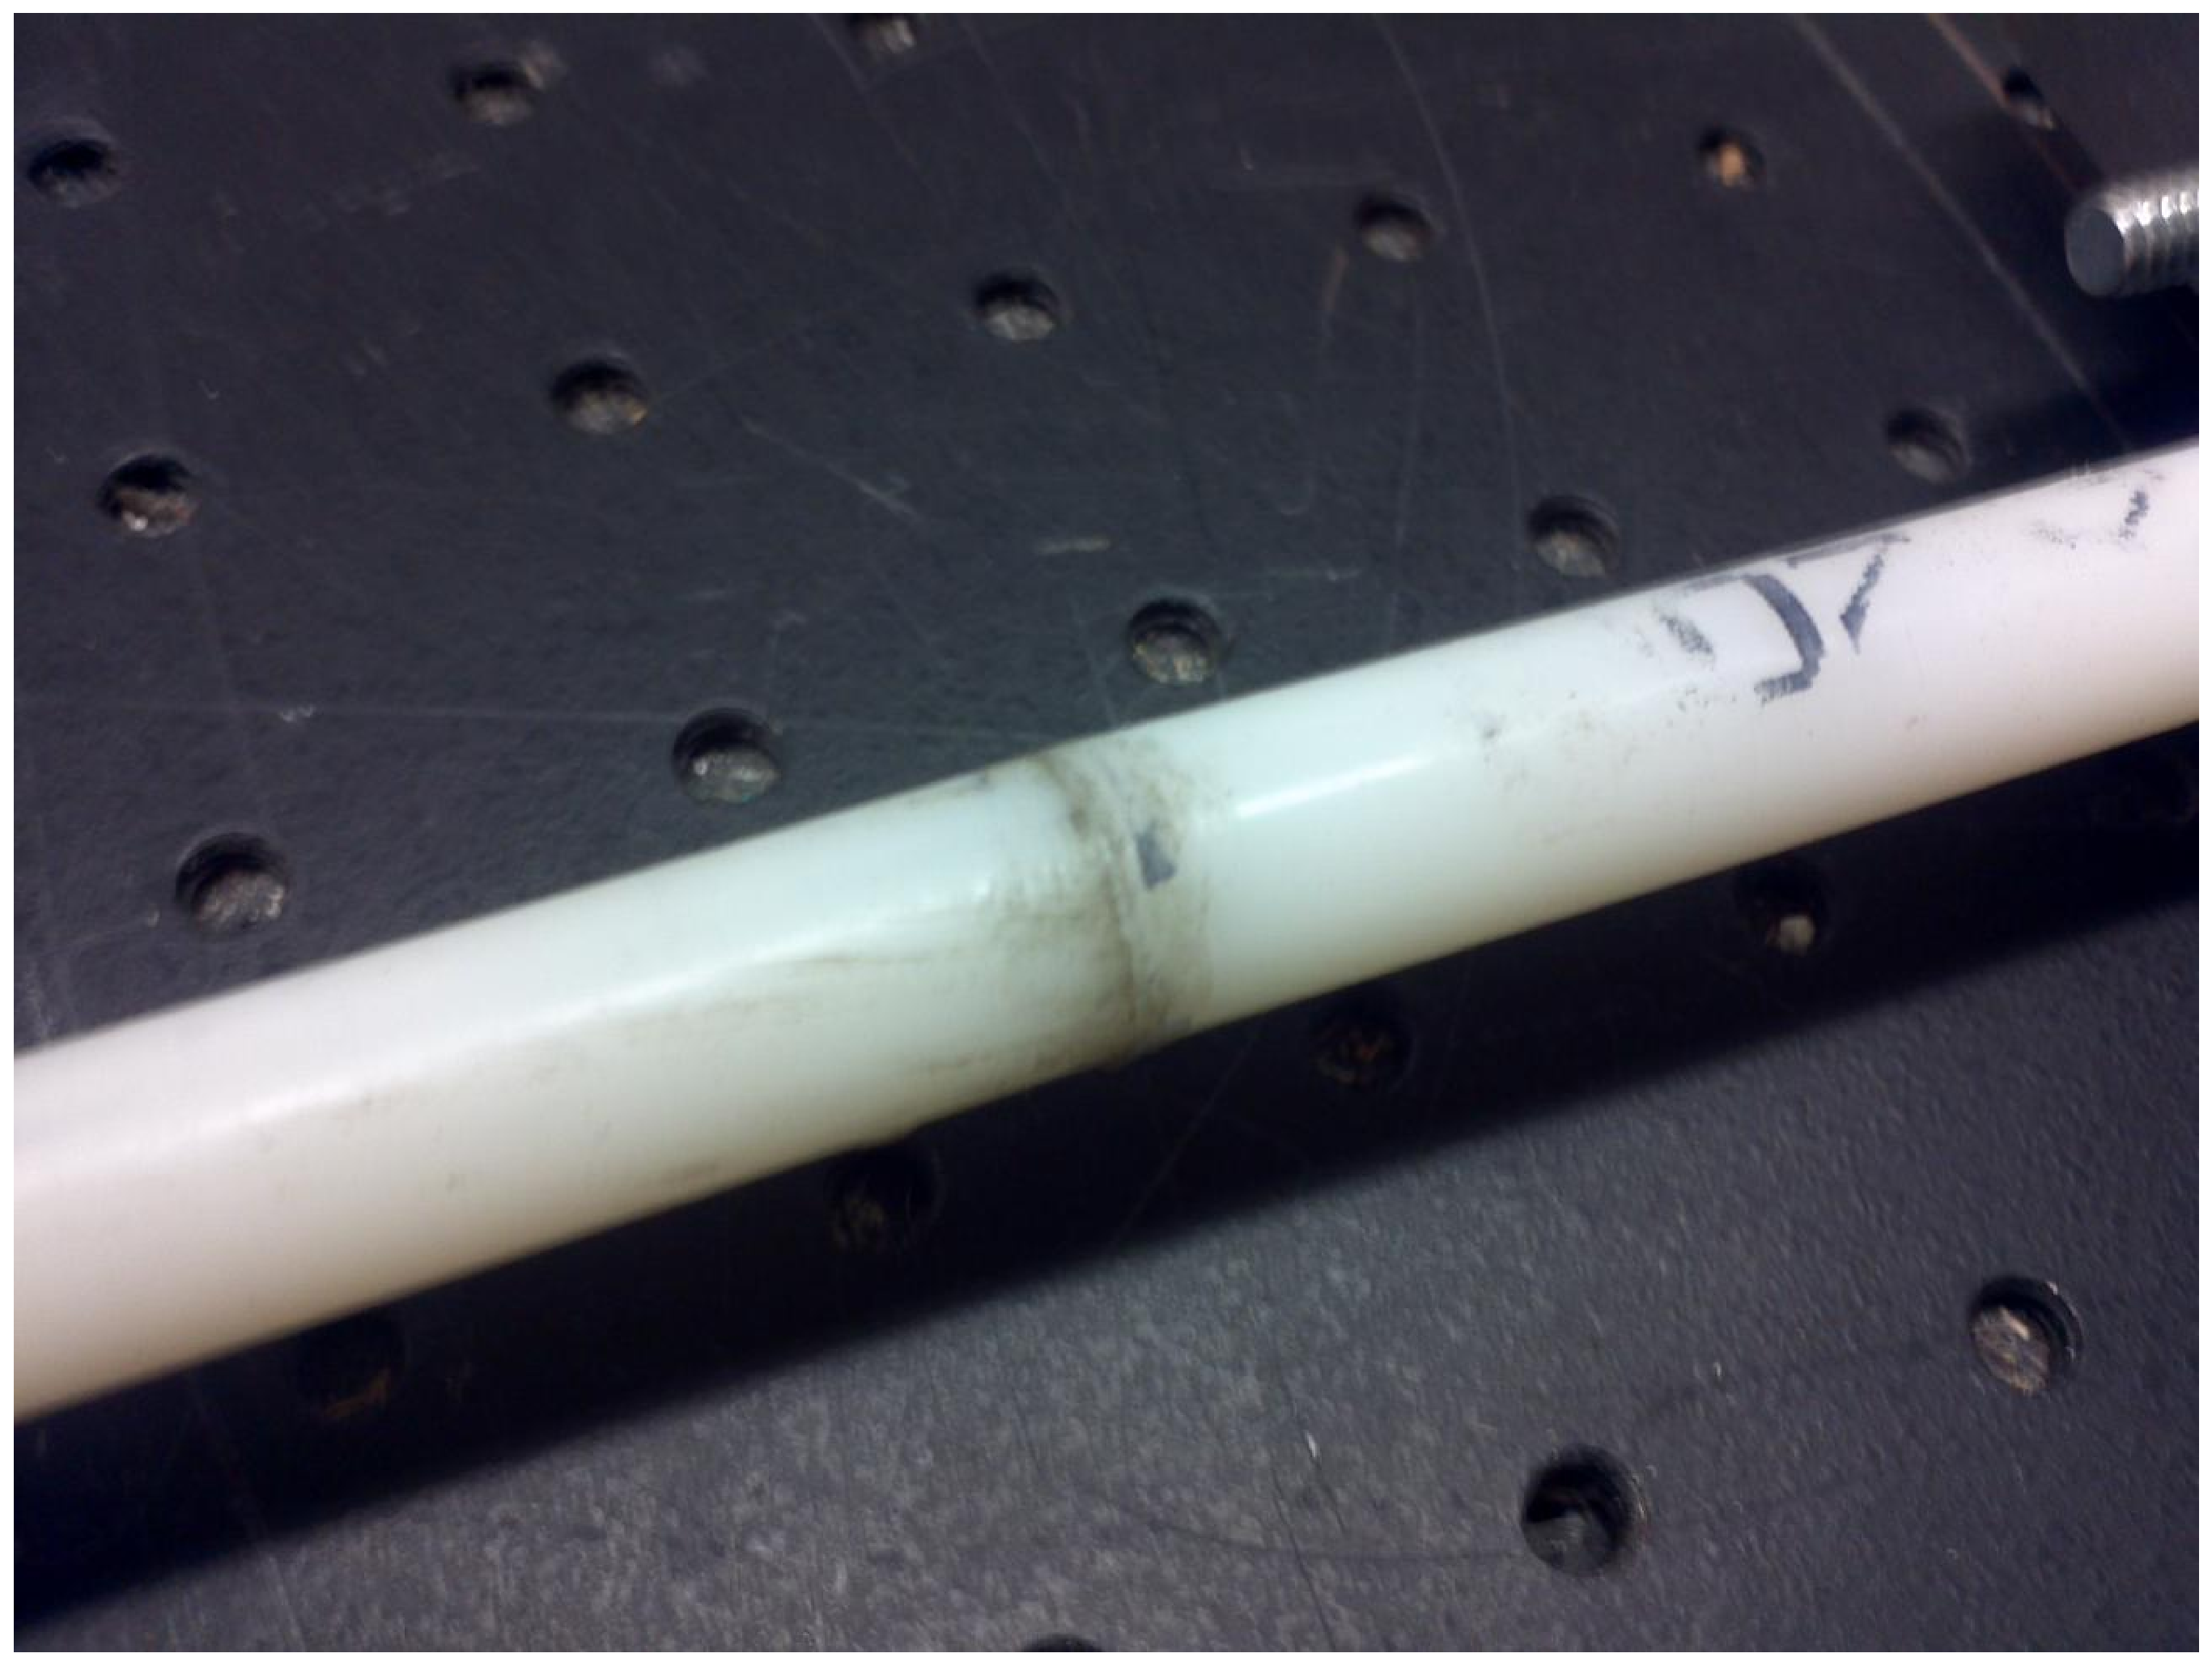
\includegraphics[width=0.6\textwidth]{eps_pics/nylonCrackClose.eps}}
\end{subfigmatrix}

   \caption[all]
%>>>> use \label inside caption to get Fig. number with \ref{}
   { \label{fig:nylonCrack}
(a) Full view of the two nylon rod pieces that are pressed together to represent a rod with a defect location.;
(b) Close up view of the defect location in the nylon rod system which should cause a noticeable change in the response at PZT B.
 }
   \end{figure}
   
\section{Time Reversal Tests}
The next step was to perform acoustic focusing at a crack located at an a priori unknown location. The tests were performed on both steel and nylon rods. The setup was very similar to that described for the crack detection tests. The main difference between these setups is that for the time reversal testing an additional PZT was placed between the two rod sections and will be referred to as the 'defect PZT'. The defect PZT acted as a defect and also provided a way to recorded the response at that location so that the overall effectiveness of the focusing algorithm could be determined. For the steel rod tests, combinations of three rod sections of different length were used which gave a total of three test combinations. The lengths of the steel rods were $579.0 \times 10^{-3} m$, $437.0 \times 10^{-3} m$, and $428.0 \times 10^{-3} m$. Similarly for the nylon rods three lengths were used which were $148.0 \times 10^{-3} m$, $105.0 \times 10^{-3} m$, and $75.0 \times 10^{-3} m$. The setup is shown schematically in Figure \ref{fig:tr_dimensions} and pictorially in Figures \ref{fig:steelTR} and \ref{fig:nylonTR}.

\begin{figure}[ht!]
\centering
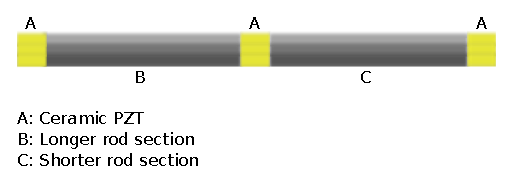
\includegraphics[width=0.8\textwidth]{eps_pics/tr_dimensions}
\caption{Schematic view of the time reversal setup. The PZTs had a length of ~$12.0 \times 10^{-3}m$. The middle PZT is referred to as the defect PZT. The two rod sections used in the tests were of different length and for generality this is just noted as 'longer' and 'shorter' section in the diagram. For the steel rods, the three lengths used were $579.0 \times 10^{-3} m$, $437.0 \times 10^{-3} m$, and $428.0 \times 10^{-3} m$ which gave a total of three combinations ($579.0 \times 10^{-3} m$ and $437.0 \times 10^{-3} m$, $579.0 \times 10^{-3} m$ and $428.0 \times 10^{-3} m$), $437.0 \times 10^{-3} m$ and $528.0 \times 10^{-3} m$). The lengths of the nylon rods used were $148.0 \times 10^{-3} m$, $105.0 \times 10^{-3} m$, and $75.0 \times 10^{-3} m$. The lengths were chosen at random and were unknown to the program during testing.
 	 \label{fig:tr_dimensions}} 
\end{figure}

\begin{figure}
\begin{subfigmatrix}{2}
\subfigure[Full view of steel rod time reversal tests]
{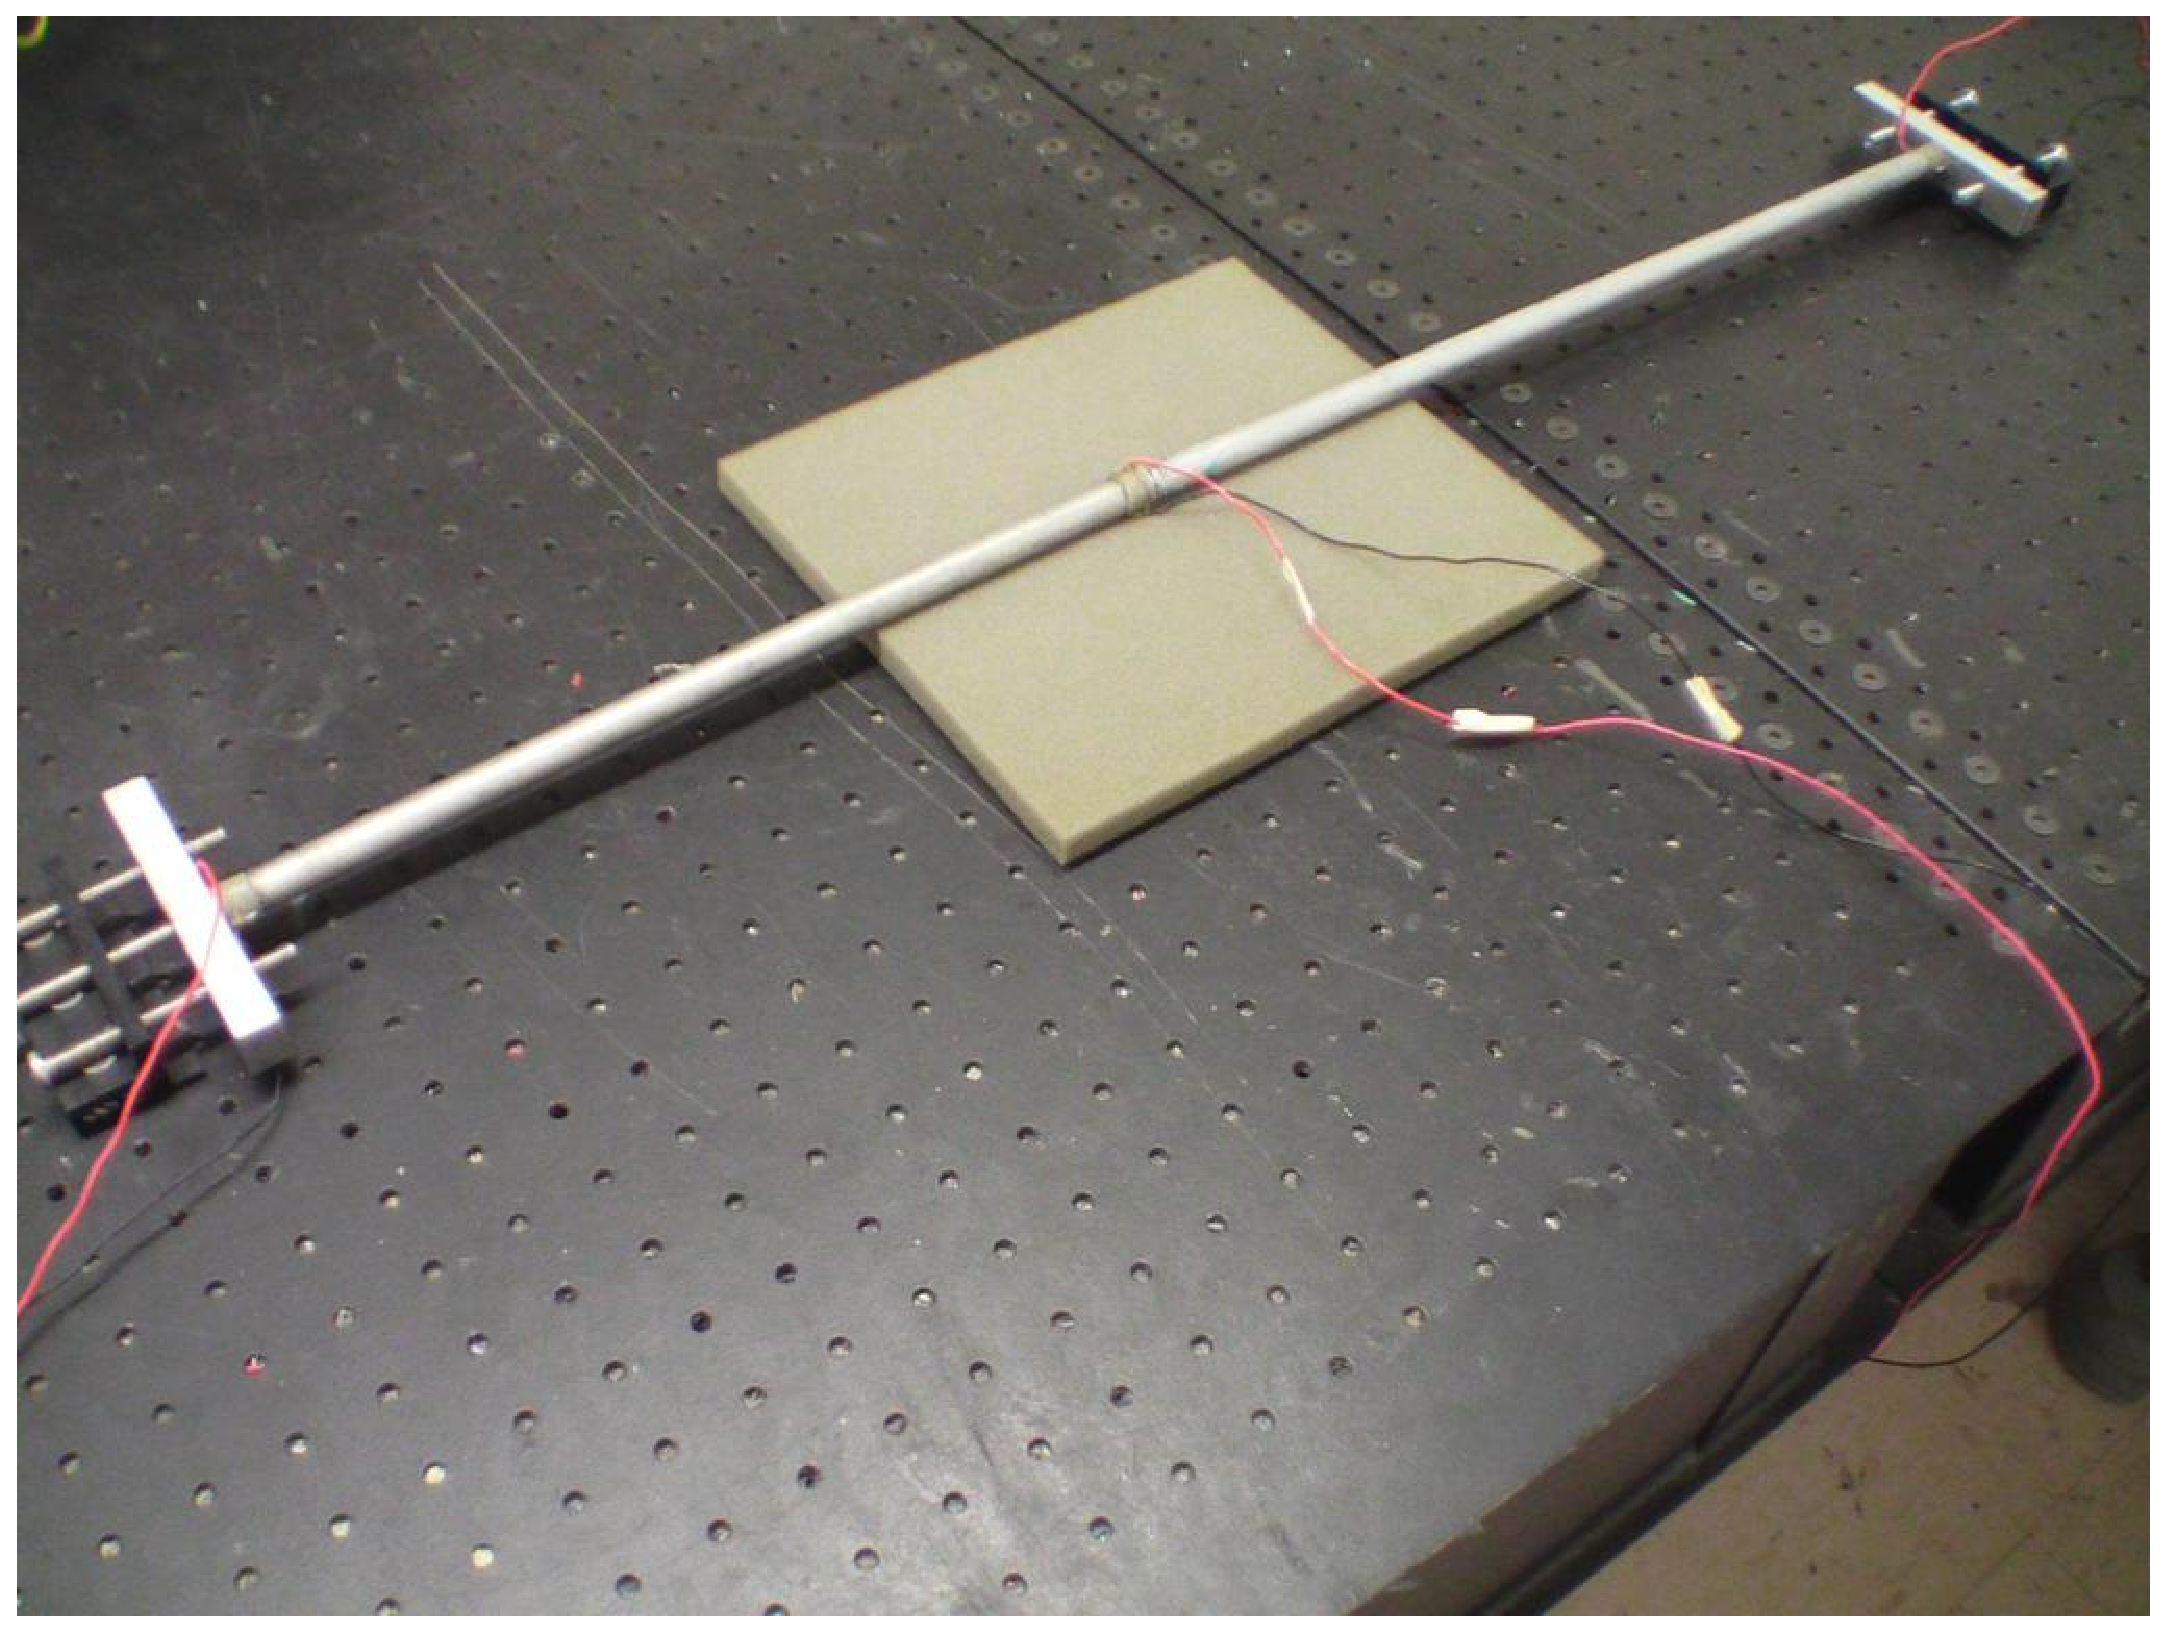
\includegraphics[width=0.6\textwidth]{eps_pics/steelSetupFull}}
\subfigure[Close up of steel rod time reversal tests]
{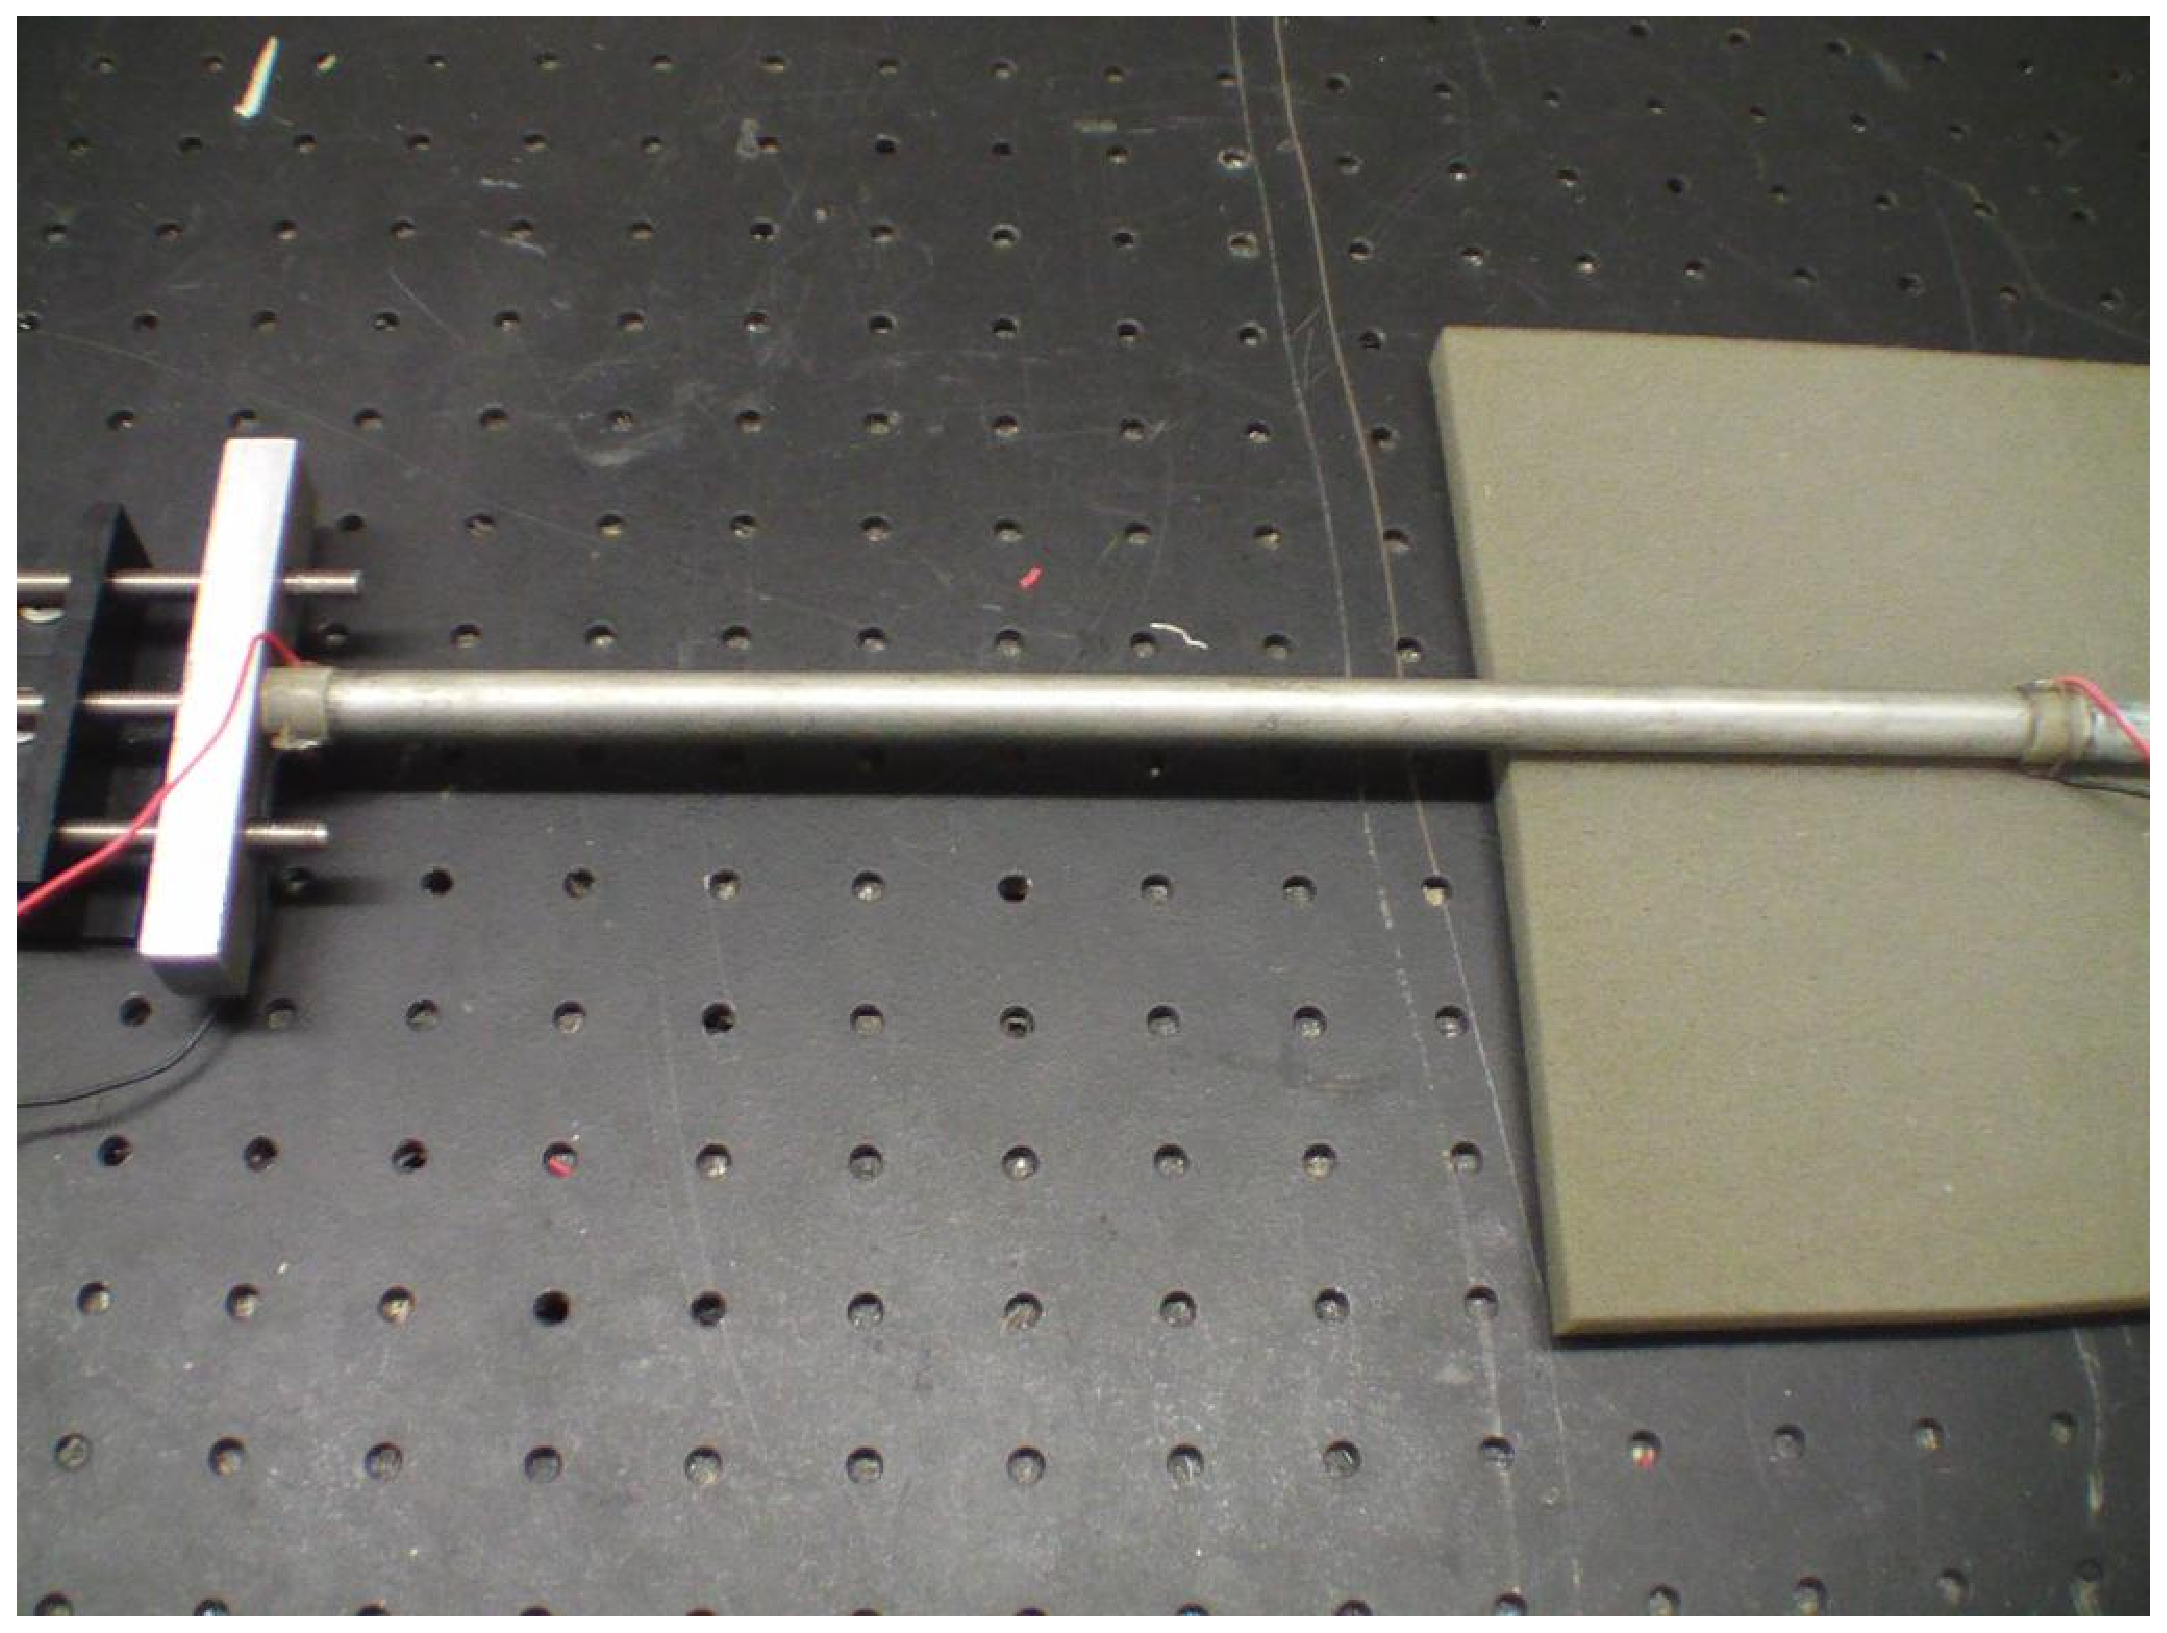
\includegraphics[width=0.6\textwidth]{eps_pics/steelSetupClose}}
\end{subfigmatrix}

   \caption[all]
%>>>> use \label inside caption to get Fig. number with \ref{}
   { \label{fig:steelTR}
(a) One set of steel rods that were used for testing;
(b) Closer view of the left side steel rod (shorter rod) section. The PZT on the right in (b) was the defect PZT and the PZT on the left in (b) was PZT B (not shown is PZT A).
 }
   \end{figure}
   
\begin{figure}
\begin{subfigmatrix}{2}
\subfigure[Full view of steel rod time reversal tests]
{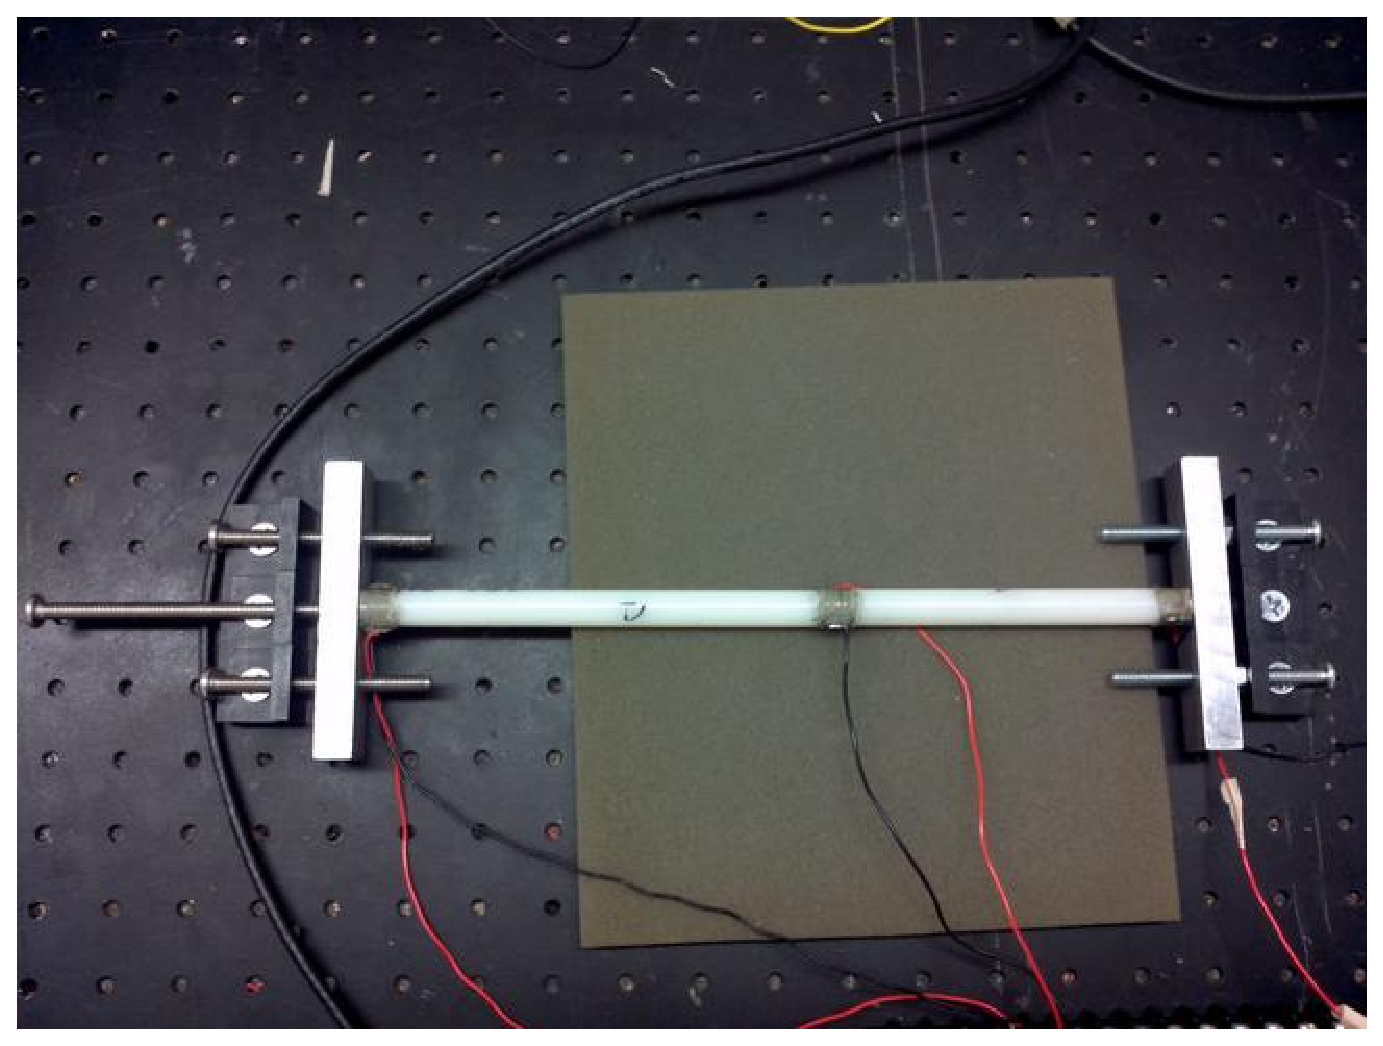
\includegraphics[width=0.6\textwidth]{eps_pics/nylonSetupFull}}
\subfigure[Close up of steel rod time reversal tests]
{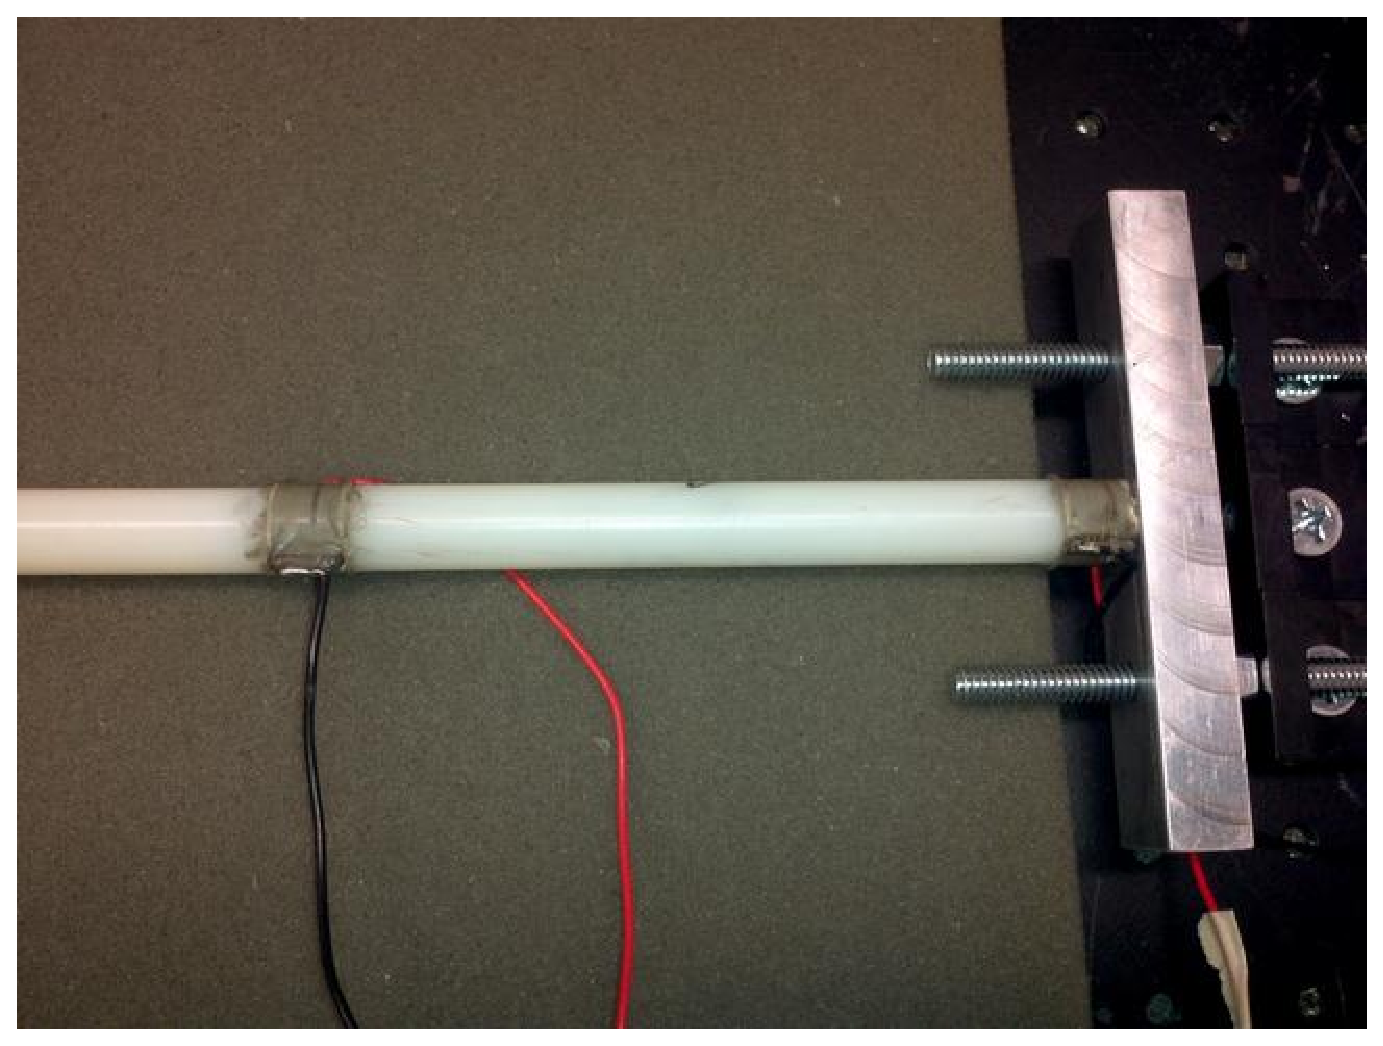
\includegraphics[width=0.6\textwidth]{eps_pics/nylonSetupClose}}
\end{subfigmatrix}

  \caption[all]
%>>>> use \label inside caption to get Fig. number with \ref{}
  { \label{fig:nylonTR}
(a) One set of nylon rods that were used for testing;
(b) Closer view of the right side steel rod (shorter rod) section. The PZT on the left in (b) was the defect PZT and the PZT on the right in (b) was PZT A (not shown is PZT B).
}
\end{figure}

The first part of the time reversal algorithm is the interrogatory phase. As with the crack detection tests, the host program generated an initial multi-tone wave that was to be played out by PZT A (although the algorithm was indifferent to which PZT plays the initial signal). Before playing out the wave the FPGA zeroed its output values and waited the specified period ($200ms$ here). PZT A sent the wave and simultaneously began recording data. Both the defect PZT and PZT B began also began recording data as the wave was being played by PZT A. The signal propagated through the rod and towards PZT B. On its way to PZT B the wave struck the defect PZT. Upon impacting the defect PZT, the wave was split into multiple components part of which were reflected back towards PZT A and part which continued transmission towards PZT B. The reflected component struck PZT A where it was recorded. The transmitted component reached PZT B where it was also recorded. The components again split upon impacting the boundaries which caused more reflection and transmission components and were also recorded by PZT A and PZT B (Figure \ref{fig:initialPhaseRead}). The recording continued until the desired number of samples for the iteration was reached (2000 samples was chosen here based upon experimental observations).


\begin{figure}
\begin{subfigmatrix}{2}
\subfigure[Response recorded at PZT A in the interrogatory phase]
{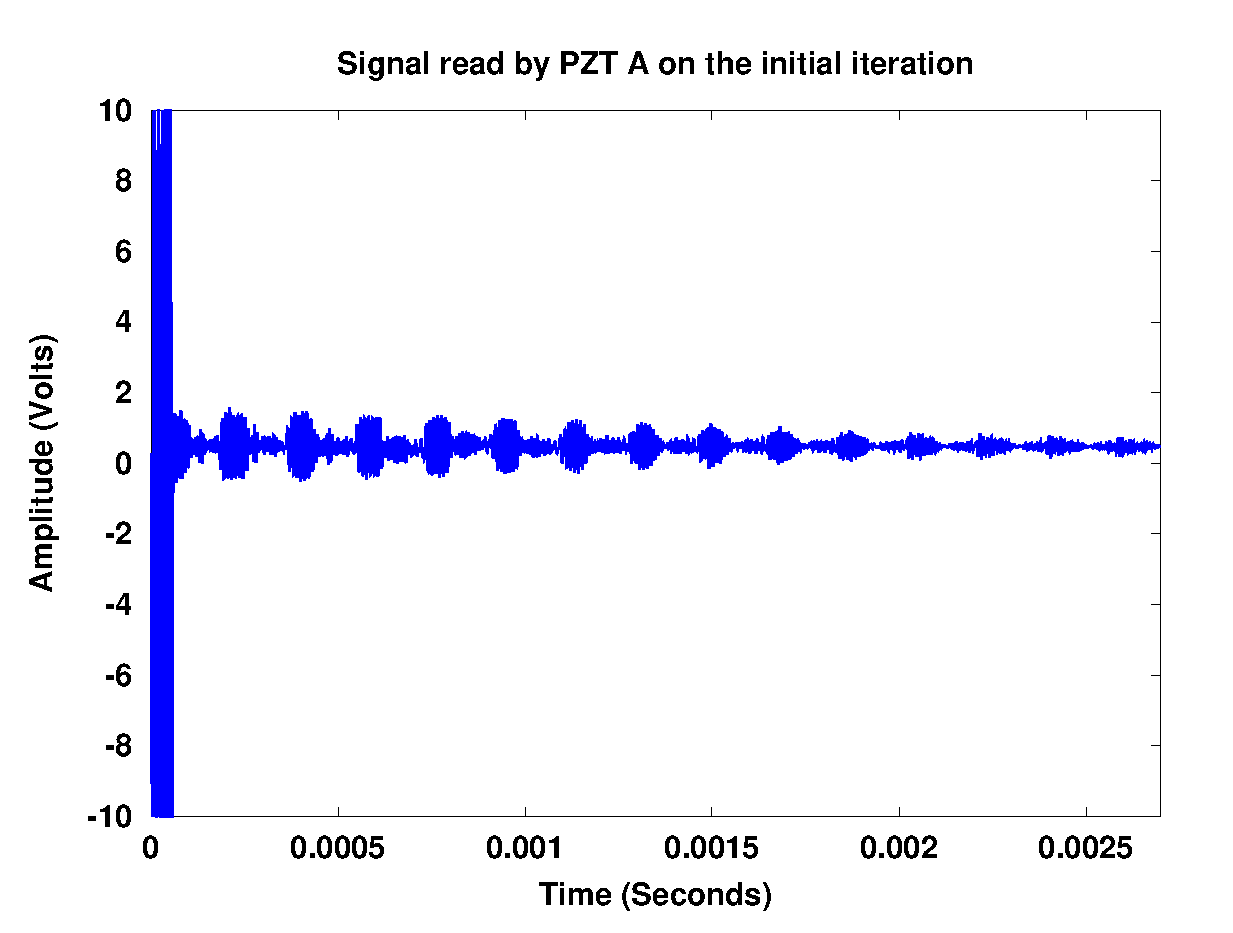
\includegraphics[width=0.6\textwidth]{eps_pics/ch0Read}}
\subfigure[Response recorded at PZT B in the interrogatory phase]
{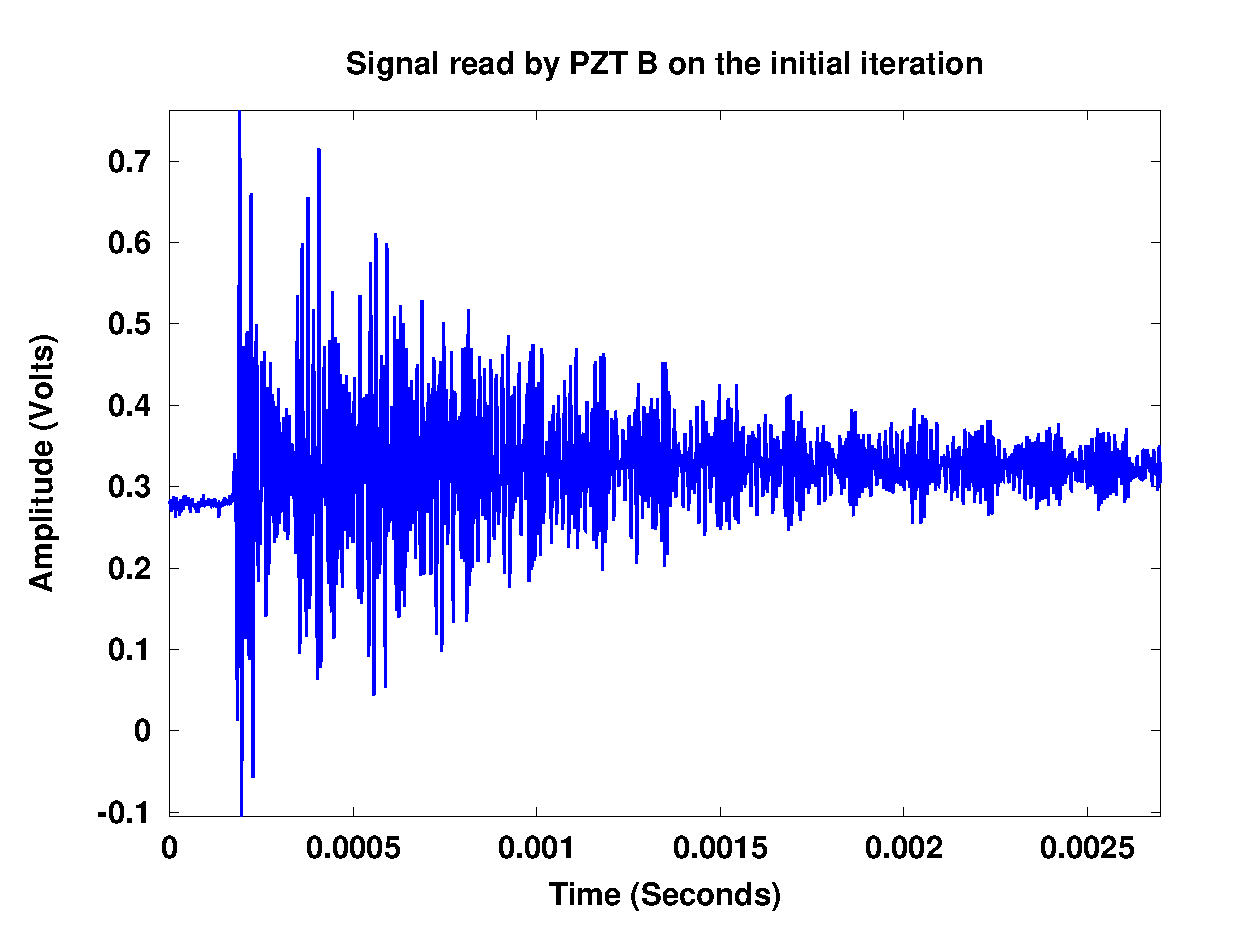
\includegraphics[width=0.6\textwidth]{eps_pics/ch1Read}}
\end{subfigmatrix}

  \caption[all]
%>>>> use \label inside caption to get Fig. number with \ref{}
  { \label{fig:initialPhaseRead}
(a) The response recorded at PZT A (sending PZT) during the interrogatory phase. These tests were carried out using steel rods which were $437 \times 10^{-3} m$ and $428 \times 10^{-3} m$ in length. It is seen that the initial wave played out by PZT A is included in the signal recorded by PZT A and is of substantially higher amplitude than the rest of the data recorded. This was one big difficulty with performing in one dimension. To make the algorithm work, it was necessary to zero out the section of the signal which contained the original wave and also to bypass ringing left over from the PZT playing the wave;
(b) The response recorded at PZT B (opposite end) during the initial iteration.
}
\end{figure}
